\documentclass[letterpaper,12pt,fullpage]{article}

\usepackage[left=1in,right=1in,top=1in,bottom=1in]{geometry}
% \usepackage{cite}
\usepackage{graphicx}
% \usepackage[dvips]{graphicx}
% \usepackage{epsfig} % for postscript graphics files
  % \graphicspath{{../eps/}}
% \DeclareGraphicsExtensions{.eps}
\usepackage{amsmath}
\usepackage{amssymb}
%\usepackage[cmex10]{amsmath}
%\usepackage{array}
%\usepackage{mdwmath}
%\usepackage{mdwtab}
%\usepackage{eqparbox}
\usepackage[tight,footnotesize]{subfigure}
%\usepackage[caption=false]{caption}
%\usepackage[font=footnotesize]{subfig}
%\usepackage{fixltx2e}
%\usepackage{stfloats}
\usepackage{hyperref}
\usepackage[backend=biber]{biblatex}
\addbibresource{exos/bleex.bib}
\addbibresource{exos/hal.bib}
\addbibresource{exos/xor.bib}
\addbibresource{exos/bodyExt.bib}
\addbibresource{exos/dualMod.bib}
\addbibresource{exos/ihmc.bib}
\addbibresource{exos/mit.bib}
\addbibresource{exos/roboKnee.bib}


% correct bad hyphenation here
%\hyphenation{op-tical net-works semi-conduc-tor}
% for LaTeX

% Single and double spacing. {\single text} or {\double text}
\newcommand{\single}{\def\baselinestretch{1.0}\large\normalsize}
\newcommand{\double}{\def\baselinestretch{1.5}\large\normalsize}
\newcommand{\triple}{\def\baselinestretch{2.0}\large\normalsize}

\def \tilde{\raisebox{-0.7 ex}{\char`\~}}
% or $\sim$

% Margin notes. \note{note to myself.}
%\newcommand{\note}[1]{\marginpar{\raggedright \small [#1]}}

% BibTex fix so \"{o} does not screw things up.
\newcommand{\dd}[1]{{\"{#1}}}

% Abbreviations for greek letters
\newcommand{\al}{{\alpha}}
\newcommand{\ep}{{\epsilon}}
\newcommand{\la}{{\lambda}}
\newcommand{\ga}{{\gamma}}
\newcommand{\om}{{\omega}}

% vectors
\newcommand{\va}{{\bf a}}
\newcommand{\vb}{{\bf b}}
\newcommand{\vc}{{\bf c}}
\newcommand{\ve}{{\bf e}}
\newcommand{\vf}{{\bf f}}
\newcommand{\vg}{{\bf g}}
\newcommand{\vh}{{\bf h}}
\newcommand{\vi}{{\bf i}}
\newcommand{\vk}{{\bf k}}
\newcommand{\vl}{{\bf l}}
\newcommand{\vm}{{\bf m}}
\newcommand{\vn}{{\bf n}}
\newcommand{\vp}{{\bf p}}
\newcommand{\vq}{{\bf q}}
\newcommand{\vr}{{\bf r}}
\newcommand{\vs}{{\bf s}}
\newcommand{\vt}{{\bf t}}
\newcommand{\vu}{{\bf u}}
\newcommand{\vv}{{\bf v}}
\newcommand{\vw}{{\bf w}}
\newcommand{\vx}{{\bf x}}
\newcommand{\vy}{{\bf y}}
\newcommand{\vz}{{\bf z}}

% Greek vectors
% We get bold greek letters from:
%\font\boldmathitalic=ambi10 at 12pt

%\newcommand{\vomega}{\hbox{\boldmathitalic !}}
%\newcommand{\vphi}{\hbox{\boldmathitalic \char'036}}
%\newcommand{\vpsi}{\hbox{\boldmathitalic \char'040}}
%\newcommand{\vtau}{\hbox{\boldmathitalic \char'034}}
%\newcommand{\vtheta}{{\bf \theta}}

% bkph's bold greek letter hack.
\def\boldify#1{\hbox{\rlap{$#1$}\kern .4pt{$#1$}}} % attempt bold Greek letter
% not needed for upper case Greek, which does come in bold! 0.6pt ?

\newcommand{\valpha}{\boldify{\alpha}}
\newcommand{\vepsilon}{\boldify{\epsilon}}
\newcommand{\vomega}{\boldify{\omega}}
\newcommand{\vpi}{\boldify{\pi}}
\newcommand{\vphi}{\boldify{\phi}}
\newcommand{\vpsi}{\boldify{\psi}}
\newcommand{\vtau}{\boldify{\tau}}
\newcommand{\vtheta}{\boldify{\theta}}

% doesn't look bold to me
% The bm package, which is part of the LaTeX tools distribution,
% defines a command \bm which may be used anywhere in maths mode. 
% \newcommand{\vpi}{{\bm \pi}}

% did not work
% this should be \boldmath \unboldmath p. 53, 201 
% \newcommand{\valpha}{{\mbox{\boldmath $\alpha$}}}

% did not work
% \newcommand{\vpi}{{\mbox{\bf $\pi$}}}

\newcommand{\vep}{{\vepsilon}}
\newcommand{\vom}{\vomega}
\newcommand{\vph}{\vphi}
\newcommand{\vps}{\vpsi}
\newcommand{\vta}{\vtau}
\newcommand{\vth}{\vtheta}

% matrices
\newcommand{\mA}{{\bf A}}
\newcommand{\mB}{{\bf B}}
\newcommand{\mC}{{\bf C}}
\newcommand{\mD}{{\bf D}}
\newcommand{\mE}{{\bf E}}
\newcommand{\mF}{{\bf F}}
\newcommand{\mG}{{\bf G}}
\newcommand{\mH}{{\bf H}}
\newcommand{\mI}{{\bf I}}
\newcommand{\mJ}{{\bf J}}
\newcommand{\mK}{{\bf K}}
\newcommand{\mL}{{\bf L}}
\newcommand{\mM}{{\bf M}}
\newcommand{\mP}{{\bf P}}
\newcommand{\mQ}{{\bf Q}}
\newcommand{\mR}{{\bf R}}
\newcommand{\mS}{{\bf S}}
\newcommand{\mT}{{\bf T}}
\newcommand{\mU}{{\bf U}}
\newcommand{\mV}{{\bf V}}
\newcommand{\mW}{{\bf W}}
\newcommand{\mX}{{\bf X}}
\newcommand{\mZ}{{\bf Z}}

\newcommand{\mOmega}{{\bf \Omega}}
\newcommand{\mPi}{{\bf \Pi}}

\newcommand{\mSigma}{\hbox{\bf \char'006}}

\newcommand{\Ep}{{E}}

\newcommand{\id}{{\bf 1}}

% transpose
\newcommand{\tr}{{\rm T}}

% probability
\newcommand{\prob}{{\mbox p}}

% variance
\newcommand{\var}{{\mbox {Var}}}

% trace
\newcommand{\trace}{{\mbox {trace}}}

% expectation
\newcommand{\E}{{\mbox {E}}}

% and, or
\newcommand{\aand}{{\mbox {and}}}
\newcommand{\oor}{{\mbox {or}}}

% argmin
%\newcommand{\argmin}{{\mbox {argmin}}}

% time handling (stolen from YTEX)
\newcount\hour
\newcount\minute
\hour=\the\time \minute=\the\time
\divide\hour by 60 \multiply\hour by 60%
\advance\minute by -\hour \divide\hour by 60%
\newcommand{\thetime}{\number\hour:\ifnum \minute<10 0\fi\number\minute}%

\newcommand{\mypsfig}[2]{\centerline{\psfig{file=#1,height=#2}}}
\newcommand{\vwhat}{\widehat{\vw}}


\newcommand{\vF}{{\bf F}}
\newcommand{\vV}{{\bf V}}
\newcommand{\vG}{{\bf G}}
\newcommand{\vT}{{\bf T}}
\newcommand{\vR}{{\bf R}}


\begin{document}

\title{A Survey of Current Exoskeletons\\ and Their Control Architectures and
Algorithms\\
(Draft 3.2)}

\author{Alex Ansari, Christopher G. Atkeson, Howie Choset, and Matthew Travers\\
Carnegie Mellon University}

\maketitle

\begin{abstract}
In the simplest case, where the environment around a robotic system remains relatively fixed, controlling the dynamic interaction between the robot and the environment to achieve a specific physical objective is difficult.  In the case where an operator effectively wears the robot, i.e., a robotic exoskeleton, and would like to move through unknown and dynamically evolving environments, the situation becomes very complicated; the robotic system needs to account for the dynamics of multiple fundamentally linked systems that are for the most part difficult to model.  The goal of this document is to provide a survey of the literature on the design, modeling, and control of robotic exoskeletons and to highlight what we believe are several of the most promising currently existing approaches to the complicated goal of enabling dynamic yet safe interaction between operators, exoskeletons, and the environment.  Where information was available, we summarize specific contributions related to actuation, power storage and generation, sensor type and distribution, mechanical architecture, as well as control system design for a number of different exoskeleton hardware systems.  Included as part of this report are recommendations on what we see as helpful components as well as potentially problematic issues in current systems and control approaches. 
\end{abstract}

\section{Executive Summary}

This paper surveys the following exoskeletons in detail:
\begin{itemize}
\item
{\bf BLEEX:} a ``minimal-sensing'' and aggressive model-based control design that has influenced many subsequent exoskeletons.
\item
{\bf HAL:} an EMG controlled exoskeleton, emphasizing recognizing operator intent.
\item
{\bf XoR:} a hybrid Pneumatic/Electric-motor system, emphasizing the
value of using multiple actuator types.
\item
{\bf Body Extender:} a fully actuated full body exoskeleton. This is the
Iron Man option.
\item
{\bf HLEE:} a nice and well presented example of a torque control approach.
\item
{\bf IHMC MAE:} an SEA-based torque controlled exoskeleton, emphasizing
the value of mixing passive mechanisms (local energy storage) and active
actuation.
\item
{\bf MIT Exoskeleton:} an attempt to take advantage of the passive dynamics
of walking.
\item
{\bf RoboKnee:} an example of a single-joint exoskeleton. Powerful single-joint
or minimal exoskeletons are one way to enable operators to move fast
and naturally, and greatly increase their strength.
\end{itemize}

We then list other exoskeletons in a variety of categories.

\section{Introduction}

This document summarizes what we have found to be several of the most relevant exoskeleton hardware systems and the associated controllers used to enable the hardware to effectively and safely interact with human operators.  As we further elaborate, the different systems that we summarize range from the relatively simple and dramatically underactuated single joint mechanisms to extremely complex and fully actuated whole-body solutions.  The controllers associated with these systems also ranged from solutions that implemented conceptually simple designs to those which made use of novel and more complex design techniques and/or relatively untried sensing and actuation technologies. 

While this document does try to provide a relatively wide overview of existing exoskeleton technology, we did focus our efforts in this report on hardware systems meant to provide power augmentation and magnification as opposed the somewhat larger subset of exoskeletons designed primarily for rehabilitation.  This choice was made relative to both hardware as well as control system design considerations.  Exoskeletons designed for rehabilitation are not typically designed as stand-alone systems and are generally limited in the scope of operational modes in which they are capable of reliably providing assistance.  The hardware designed for athletic operators and extreme tasks will need to be high-powered with a power source that is capable of being carried such that the suit is a completely stand alone unit and will need to run a control system that is capable of providing transparent support to the operator in a large variety of operational scenarios.

To this end, the hardware systems that we chose to include summaries of in this document were the BLEEX, HAL, XoR, Body Extender, Hydraulic Lower Extremety, IHMC Mobility Assist, MIT, and RoboKnee exoskeletons.  The different systems cover many of the possible choices of actuation strategies, ranging from electric motors, to hydraulics, to pneumatics, and combinations thereof.  Several of the systems used novel transmission strategies as well, focusing on both efficient as well as high-fidelity force control implementations.  The transmission strategies included standard hydraulic systems, hydraulic systems with actively controlled bypass valves, ball-screw mechanisms that include series elastic components, as well as pneumatically actuated pulley-tendon and belt-drive mechanisms. 

In terms of sensing and control technologies, the different exoskeletons covered in this report employed a wide variety of the spectrum of available options.  Sensors were used to measure everything from standard information, like angular displacement of the hardware system's joints, to more novel information, like muscle activity of the user using EMG technology.  Sensor information was used as the basis for a variety of different closed and open-loop control system designs, ranging from straight-forward force control and trajectory following to novel approaches of fully actuated feedback linearization and sensitivity amplification strategies.  

Each of these component technologies are reviewed as they relate to the hardware systems discussed in this report.  Recommendations on what we feel are the best approaches in these reviews are also provided.  We provide a summary of these recommendations at the end of this document.

%\section{Scope: What is this paper about?}
%
%This paper surveys exoskeleton control architectures and
%algorithms.
%The focus is on exoskeleton control that allows a
%highly trained and top percentile athletic 
%operator to carry a payload that weighs approximately the same amount
%as the operator. We envisage these types of exoskeletons to be useful
%in carrying protective and safety equipment for SWAT teams, police,
%firefighters, and soldiers. 
%We also 
%focus this survey on exoskeleton control for lower body tasks (standing, walking,
%running, jumping, kicking, dodging, ...).

\section{BLEEX}
\label{exo:bleex}

keywords: sensitivity amplification; strength augmentation.\\

The Berkeley lower extremity exoskeleton (BLEEX) is an anthropomorphic, powered exoskeleton designed for human strength augmentation.  It is described as the first field-operational robotic system to allow its operator to carry significant loads over unstructured terrain without external power \cite{bleex_design_2006}.

\begin{figure}[ht]
  \centering
  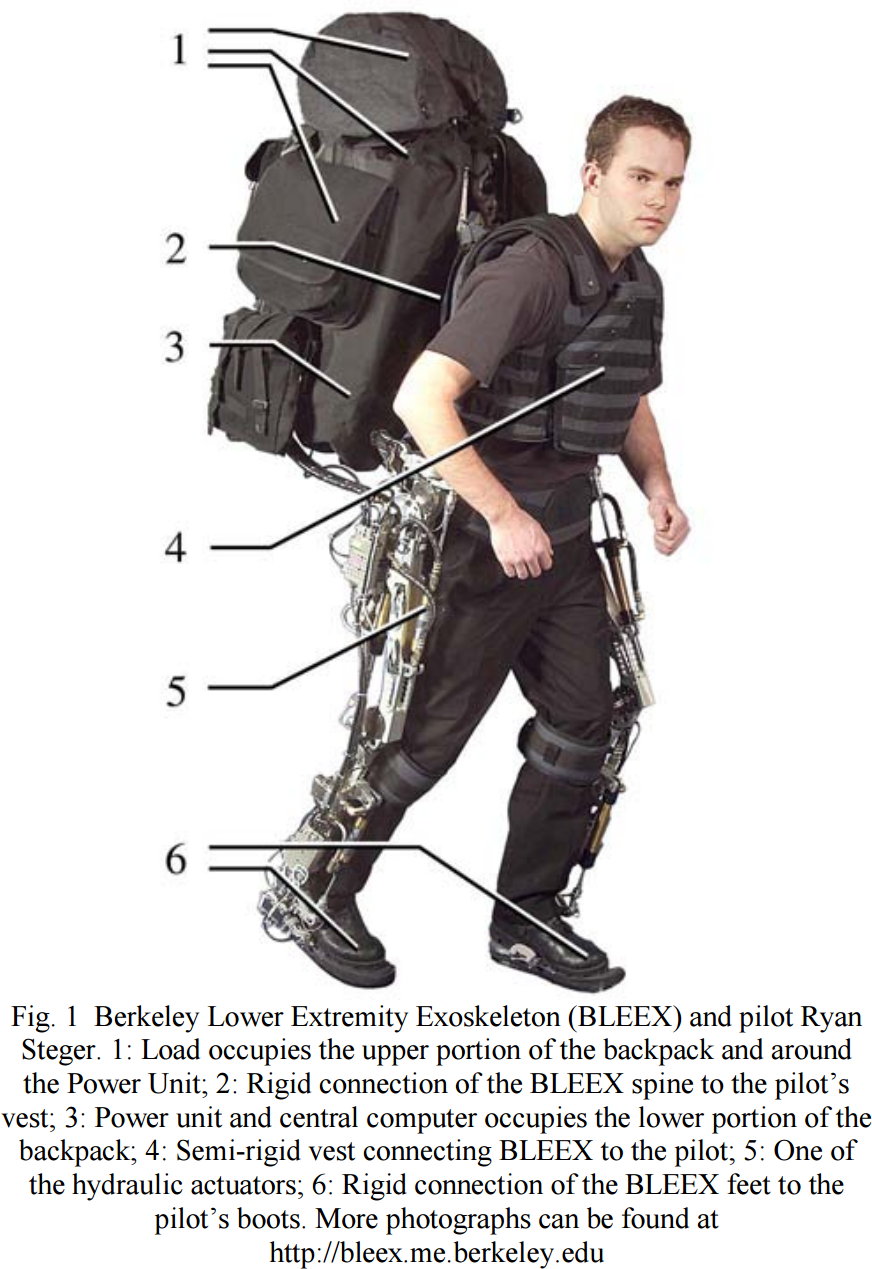
\includegraphics[width=3.5in]{exos/figs/bleex_exo.png}
\end{figure}

The BLEEX system includes two 7 DOF, three-segment legs with thigh, shank, and foot links, on-board power supply, and a backpack-like frame.  The human wearer is rigidly connected at the feet and torso such that the frame shelters the user by transferring load forces to the ground.  The leg segments are connected by rotational joints including 3 DOF (2 actuated) at the hip, 1 DOF (actuated) at each knee, and 3 DOF (1 actuated f/e in sagittal 
plane; 2 passive) at the ankles.  Joint angles, torque, and power requirements are determined from human motion analysis based on a 75-kg human walking on flat ground at roughly 1.3 m/s (the average military male's maximum reported joint limits are also used to derive joint range of motion targets).  During design, joint motion was intended to be slightly less than the maximum human range of motion for safety; however, some joint ranges had to be reduced to avoid singularities.
% Ideally, joint motion would provide the maximum human range of motion for safety

Due to its high power to weight ratio (twice that of electric motors), BLEEX uses a hydraulic actuation system.  An on-board internal combustion engine provides both electric and hydraulic power.  The joints are driven by commercial small bore (2cm) dual action hydraulic actuators operating at 6.9 MPa. Though the operating pressure is relatively low, the hydraulic actuation system exhibits significant pressures losses across servo valves when less pressure is required than this system pressure.  Table~\ref{tab:bleex_joints} provides details regarding the range of motion and torque capabilities of BLEEX's joints.  As reported in \cite{bleex_design_2006}, BLEEX requires 1,143 W for walking relative to 165 W for human walking (14\% efficient compared to a human of the same size).  Altogether the suit needs 2.27 kW of hydraulic power and 220 W of electric power to accommodate climbing (540 W) and remaining electrical loads including 240 W to power the second stages on servo vales.

%
\begin{table}
\centering
\begin{tabular}{|l|*{3}{c|}}  % repeats {c|} 6 times
\hline
& BLEEX & human max & BLEEX \\
& ROM & torque \& power & max torque \\ \hline
Ankle flexion / extension & $\pm 45^\circ$ & $-120$ N-m; 250 W & $-200 / 155$ N-m\\ \hline
Ankle abduction / adduction & $\pm 20^\circ$ & N/A & N/A \\ \hline
Knee flexion & $121^\circ$ & $-35 / 60$ N-m; $-150 / 50$ W & $-100 / 140$ N-m \\ \hline
Hip flexion / extension & $\pm 121^\circ / 10^\circ$ & $-80 / 60$ N-m; $-60 / 115$ W & $-150 / 130$ N-m \\ \hline
Hip abduction / adduction & $\pm 16^\circ$ & N/A & N/A\\ \hline
total rotation external & $35^\circ$ & N/A & N/A \\ \hline
total rotation internal & $35^\circ$ & N/A & N/A \\ \hline
\end{tabular}
\caption{BLEEX joint range of motion (ROM) is near anthropomorphic.  The max torques are designed to meet the torque / power requirements of similarly sized human walking at 1.3 m/s \cite{bleex_design_2006}.}\label{tab:bleex_joints}
\end{table}
%

\subsubsection{Control}

The BLEEX team has successfully implemented both sensitivity amplification \cite{sesitivityAmpPaper2005} and a hybrid assitive control scheme \cite{bleex_hybrid_control_2006} that switches (based on gait phase) between sensitivity amplification and a position control regulating desired torque. This section focuses on sensitivity amplification, as the hybrid assitive strategy did not perform as well in walking trials.

\begin{figure}[ht]
  \centering
  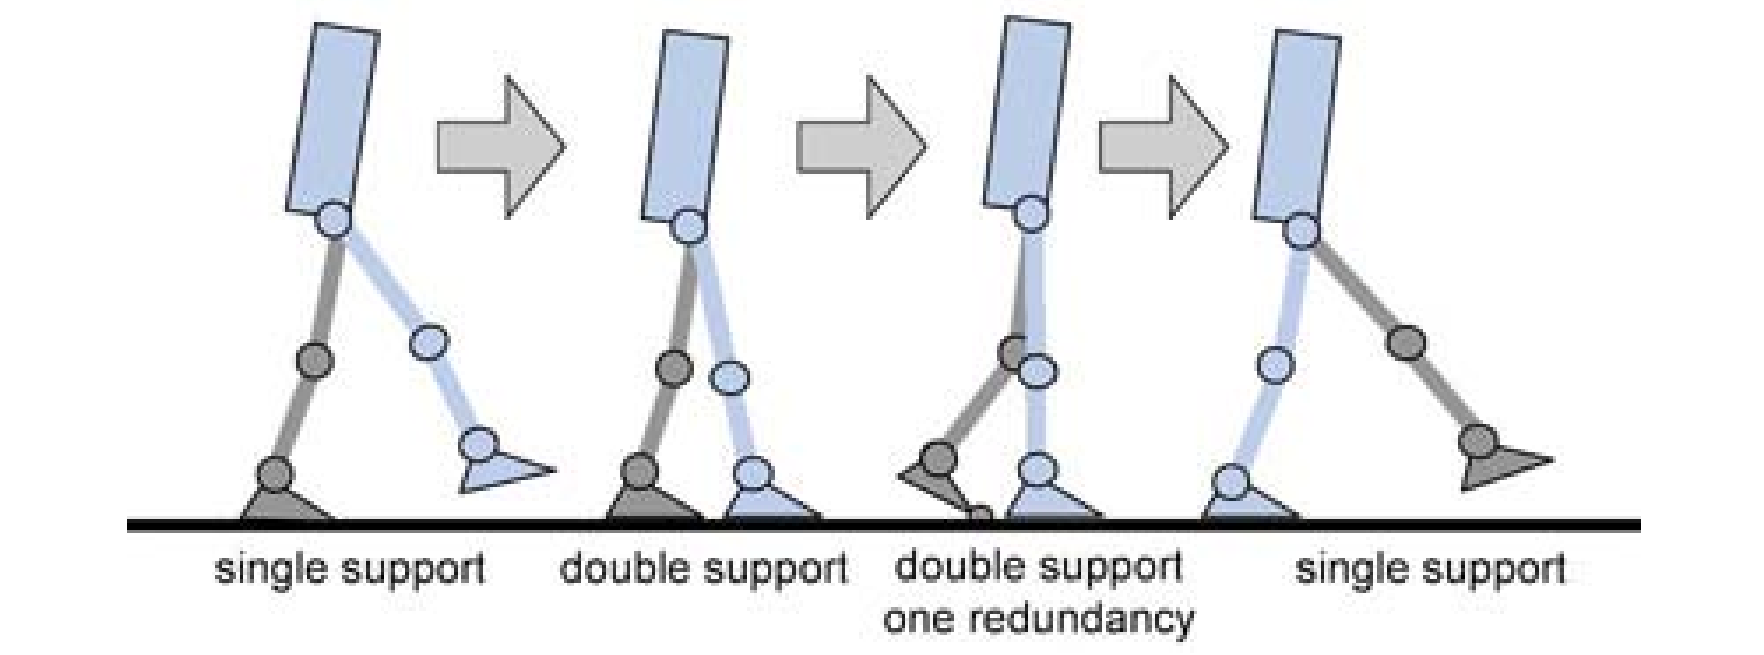
\includegraphics[width=3.5in]{exos/figs/bleex_support_phases.png}
\end{figure}

In its sensitivity amplification implementation, BLEEX controllers attempt to minimize interaction forces between the human pilot and the exoskeleton. However, the BLEEX team makes a point to avoid direct measurements of the interaction force between the human and the exoskeleton suit.  They highlight difficulties in properly outfitting humans with necessary sensing equipment and challenges in modeling the interaction between the human and exoskeleton (e.g., non-rigid, non-fixed contact points).  Instead, the team develops controllers based on an inverse dynamic model (in the saggital plane) of only the exoskeleton.  

\begin{figure}[ht]
  \centering
  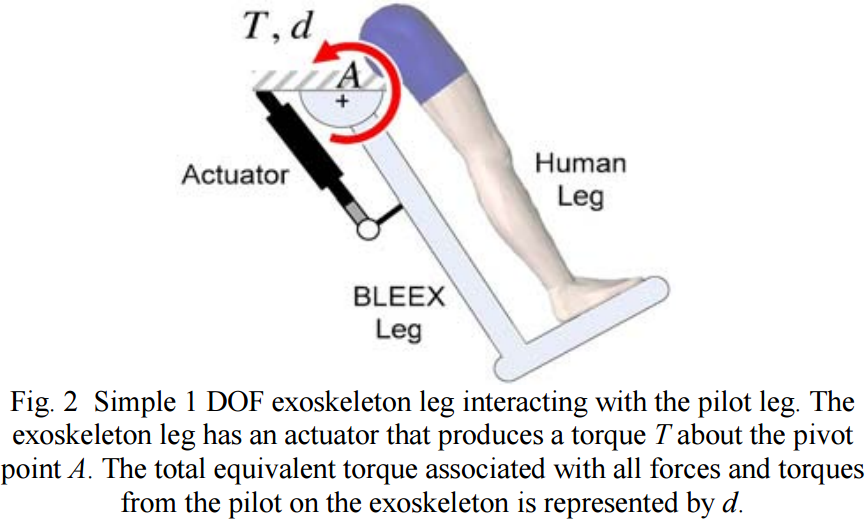
\includegraphics[width=3.5in]{exos/figs/bleex_1dof_ex.png}
\end{figure}

Assuming no outside disturbances, the BLEEX sensitivity amplification control strategy models the torque applied by the human pilot on the exoskeleton as $d$ (assuming no outside disturbances).   Neglecting gravity, the exokeleton angular velocity is modeled as 
\[v = G r + S d ,\] 
where $v$ represents the angular velocity of the exokeleton, $G$ is the transfer function from actuator inputs ($G$ is the exoskeleton's dynamics), $r$ is the actuator input, and $S$ is the sensitivity or transfer function from human torque to exokeleton angular velocity. 

\begin{figure}[ht]
  \centering
  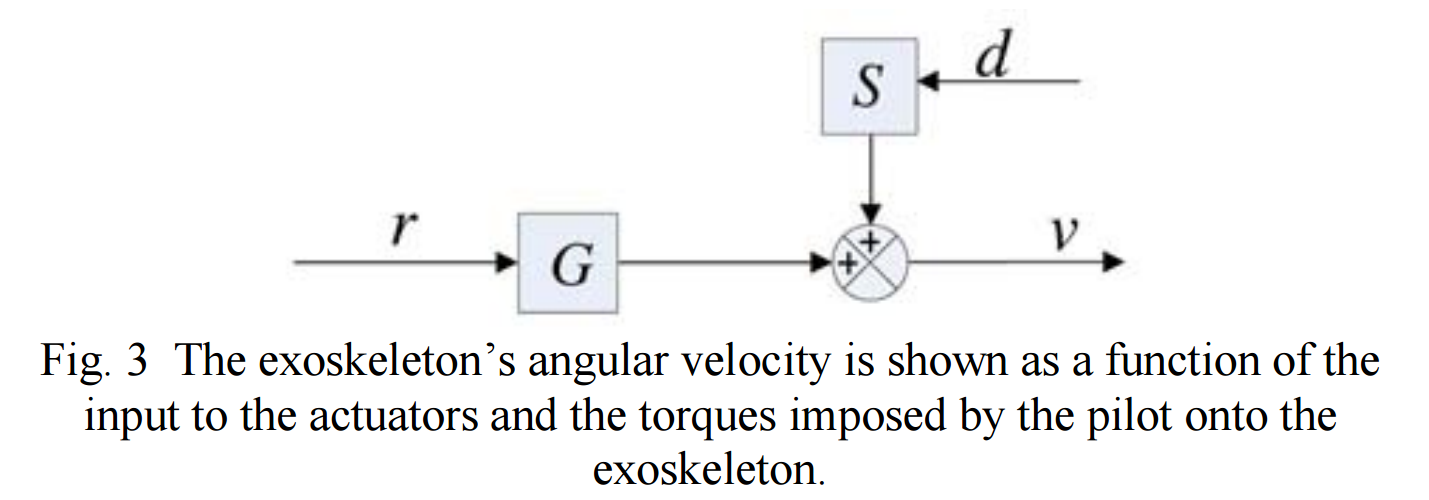
\includegraphics[width=4.0in]{exos/figs/bleex_control_diag_1.png}
\end{figure}

The goal is to maximize sensitivity to $d$ \emph{without direct measurement.}  Sensitivity amplification accomplishes this by creating a feedback loop from a controller, $C$, acting only on exoskeleton variables.  A new sensitivity equation,
\[S_{new} = \frac{v}{d} = \frac{S}{1 + G C} ,\]
is maximized by applying positive feedback.  To achieve a large sensitivity, BLEEX uses $C = (1-\alpha^{-1})G^{-1}$ so that $\alpha$ provides a direct (scalar) amplification factor. A low pass filter is often added to the $C$ term in order to damp out high frequency dynamics of the exoskeleton, which are not captured in these models.  Note that the controller depends on an inverse dynamic model of the exoskeleton, $G^{-1}$.  Since the model is hybrid, these dynamics switch according to gait phases (single support, double support, stance).  BLEEX detects these transitions using foot sensors.  Assuming the single leg support dynamics are in the form,
\begin{equation}
\mM({\bf\theta})\ddot{{\bf \theta}} + \mC({\bf\theta},\dot{{\bf\theta}}) \dot{{\bf \theta}} + \mV({\bf\theta}) = {\bf T} + {\bf d} ,
\end{equation}
where ${\bf T}$ is a vector of actuator torques, the BLEEX control torque would be
\begin{equation}
{\bf T} = \mV({\bf\theta}) + (1 - \alpha^{-1}) \big [ \mM({\bf\theta})\ddot{{\bf \theta}} + \mC({\bf\theta},\dot{{\bf\theta}}) \dot{{\bf \theta}} \big ] .
\end{equation}
The user must provide the first torque component as the exoskeleton has no actuator acting between the foot and the ground (the system is underactuated).

\begin{figure}[ht]
  \centering
  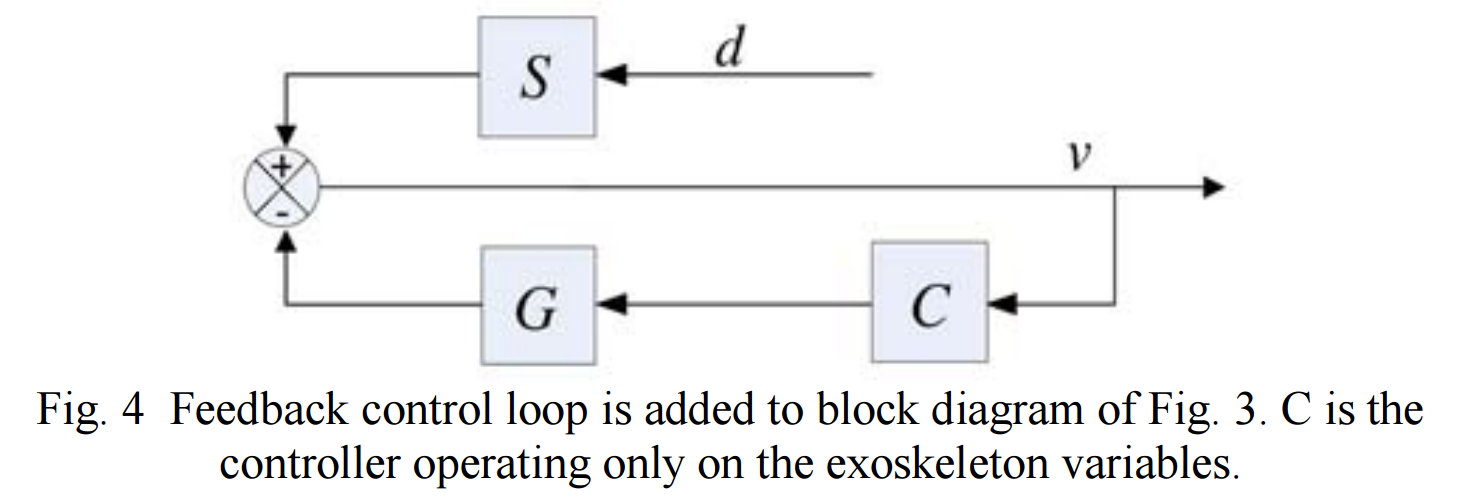
\includegraphics[width=4.0in]{exos/figs/bleex_control_diag_2.png}
\end{figure}

As a note, positive feedback is normally avoided in control design because it amplifies disturbances.  In the case of BLEEX, designers sacrifice disturbance rejection to maximize the response of the suit to its wearer.  Users must therefore take action to stabilize and balance out disturbances.

\begin{figure}[ht]
  \centering
  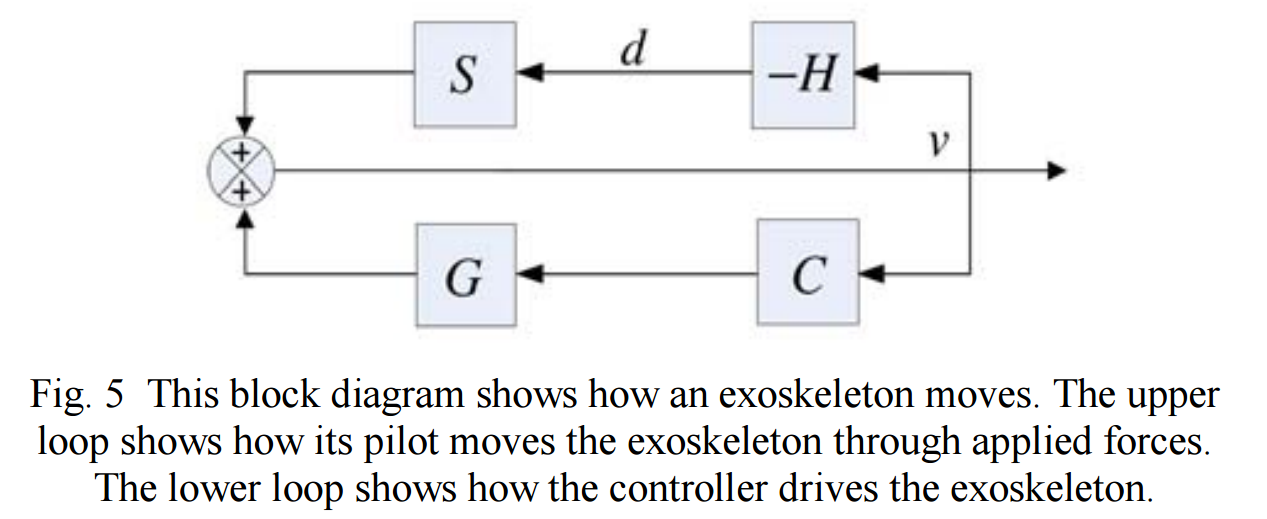
\includegraphics[width=4.0in]{exos/figs/bleex_control_diag_3.png}
\end{figure}

For sensing, BLEEX uses information from \textbf{8 encoders} and \textbf{16 accelerometers} to determine angle, angular velocity, and angular acceleration of eight actuated joints. It includes a \textbf{foot switch and load distribution sensor} at each foot. Eight single axis \textbf{force sensors} provide measurements required to perform low level force control at each actuator. An \textbf{inclinometer} indicates the orientation of the backpack relative to gravity. Using this sensitivity amplification control scheme, BLEEX has achieved successful walking at 1.3 m/s with a 34kg payload \cite{sesitivityAmpPaper2005}.

\subsection{Assessment and Recommendations}

Sensitivity amplification is a current best-in-class control strategy.  The exoskeleton shadows the user and uses exoskeleton data for joint angle, velocity, and acceleration and the exoskeleton model to minimize torques experienced by the human torque.  The process and hardware are relatively simple yet effective.   However, the approach has several significant disadvantages including heavy reliance on an accurate exoskeleton model and the fact that sensitivity amplification will amplify disturbances.  Note that in combat situations this latter point is critical as a sensitivity amplification will amplify forces acting on the suit and the operator will have to re-act to compensate.  The only way to compensate for or resist external forces in this setting is to filter them out, which would be extremely challenging unless additional sensory equipment is provided.  As one possibility, a sensitivity optimization approach may be paired with sEMG data to estimate user intent and provide such a filter.  Note this type of implementation would present its own challenges considering limitations in sensing and calibration of current EMG systems. 


\bibliographystyle{plain}
\bibliography{exos/bleex}

The figures in this section were obtained from \cite{sesitivityAmpPaper2005}. Materials presented are based on the references above.


\section{HAL}
\label{exo:hal}
\begin{refsection}[exos/hal.bib]

% keywords: model-based control; predefined gait trajectory; strength augmentation; rehabilitation.\\

The hybrid assistive limb (HAL) exoskeleton is developed by the University of Tsukuba and Cyberdyne for human strength augmentation and as an assistive gait device in rehabilitation.  Although several prototypes have been developed, this section focuses on the most recent HAL-5 model (specifically the non-clinical type, HAL-5 Type-B). Though HAL-5 is a full body exoskeleton, only hip, knee joints, and ankle are actuated in the sagittal plane.  The exoskeleton uses DC motors with harmonic drives at hip, knee, ankle joints (in some models the ankle joints act as passive springs).  HAL weighs 23kg and includes an on-board AC100V battery as the power source, which is designed to support maximum velocity human walking and standing torque requirements.  The battery allows for 160 min of continuous operation and enables the exoskeleton to lift up to 70kg \cite{HALassist2011}.  

Human operators attach to HAL at the waist with a belt, and at the calf and thigh using harnesses. HAL's frame does not transfer load to the ground.  Instead, HAL adjusts hip, knee and ankle torques to amplify its operator's torque. The exoskelton's sensory system includes bioelectric sensing (including \textbf{sEMG}), \textbf{angular sensors}, \textbf{acceleration sensors}, and \textbf{center of pressure / center of gravity} (COP/COG) sensors.  COP/COG sensing is provided through shoes with ground reaction force sensors.  The joint measurements are provided by potentiometers.
In at least one version of HAL the bioelectric data comes from sEMG sensors installed below the operator's hip and above the knee (on both front and back).
An IMU installed in HAL's backpack is used to estimate torso pose.


\begin{figure}[ht]
  \centering
  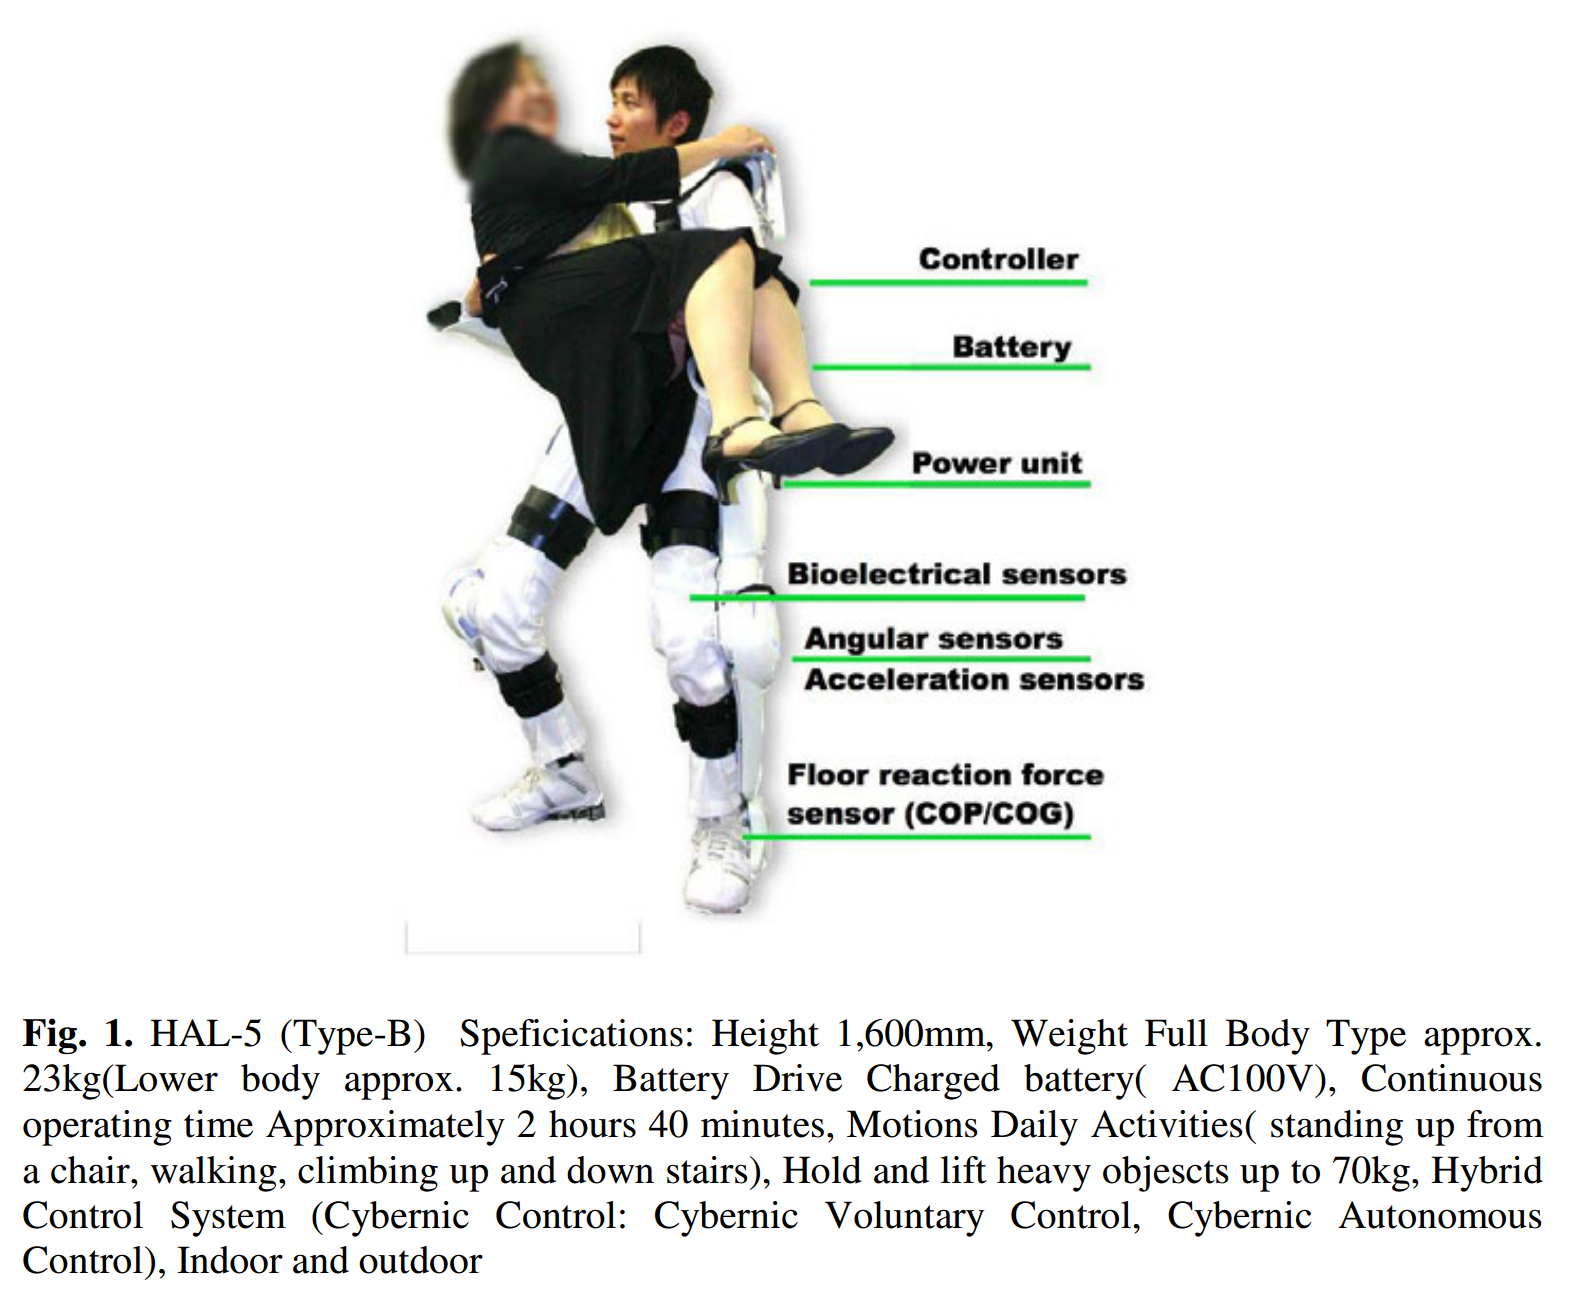
\includegraphics[width=3.5in]{exos/figs/hal-5_B_diagram.png}
\end{figure}


\subsubsection{Control}

HAL has two types of control systems designed for different application domains.  For gait assistance and rehabilitation, HAL uses an autonomous control system that carries the user through predefined gait trajectories by controlling knee and hip joints (the ankles behave as passive springs).  Gait phase intention is estimated from COP/COG sensors.  The exoskeleton drives the wearer to follow pre-recorded desired joint patterns.

The second control strategy, a model-based approach for human strength augmentation, estimates human intention from sEMG activity and provides power to augment torque provided by the operator.  A relatively autonomous torque assist strategy in \cite{HALmodelControlKnee2010} recognizes user intention to take a step by thresholding sEMG data.  The approach provides a knee torque response including an assitive torque component, a viscous damping component that reduces high velocity motion for safety, and a gravity compensation torque.  
%In \cite{HALvTorqueImp2002}, HAL uses myoelectric data to estimate muscle torque based on the difference between flexor and extensor muscle activities.  

In \cite{HALmuscleImped2005}, an impedance control strategy controls the viscoelastic properties of HAL's knee joint from a musculoskeletal model of operator's limb moving in concert with the exoskeleton.  The controller uses sEMG sensor data to estimate muscle torque based on the difference between flexor and extensor muscle activities.  The authors note the sEMG model requires significant calibration effort.  
Viscoelastic torques are computed according to
\[\tau_{a,i} = \alpha_i(-D_i \theta_i - K_i \theta_i),\]  
based on a variable gain set by $\alpha_i$.  The net knee actuator torque is
\[\tau_i = \tau_{a,i} + \tau_\mu + \tau_c .\]
The torque includes a $\tau_c$ term compensating for mechanical (actuator) impedance and $\tau_\mu$, a scaled version of the human torque (as estimated  from sEMG data).  The $K_i$ and $D_i$ terms in $\tau_{a,i}$ are viscoelastic parameters (based on the operator's muscles) in the human-exoskeleton model.  These parameters are estimated on-line using a weighted least-squares method.  In this case, the angular velocity data required for the impedance controller is estimated from a state observer.

%
\begin{figure}[ht]
  \centering
  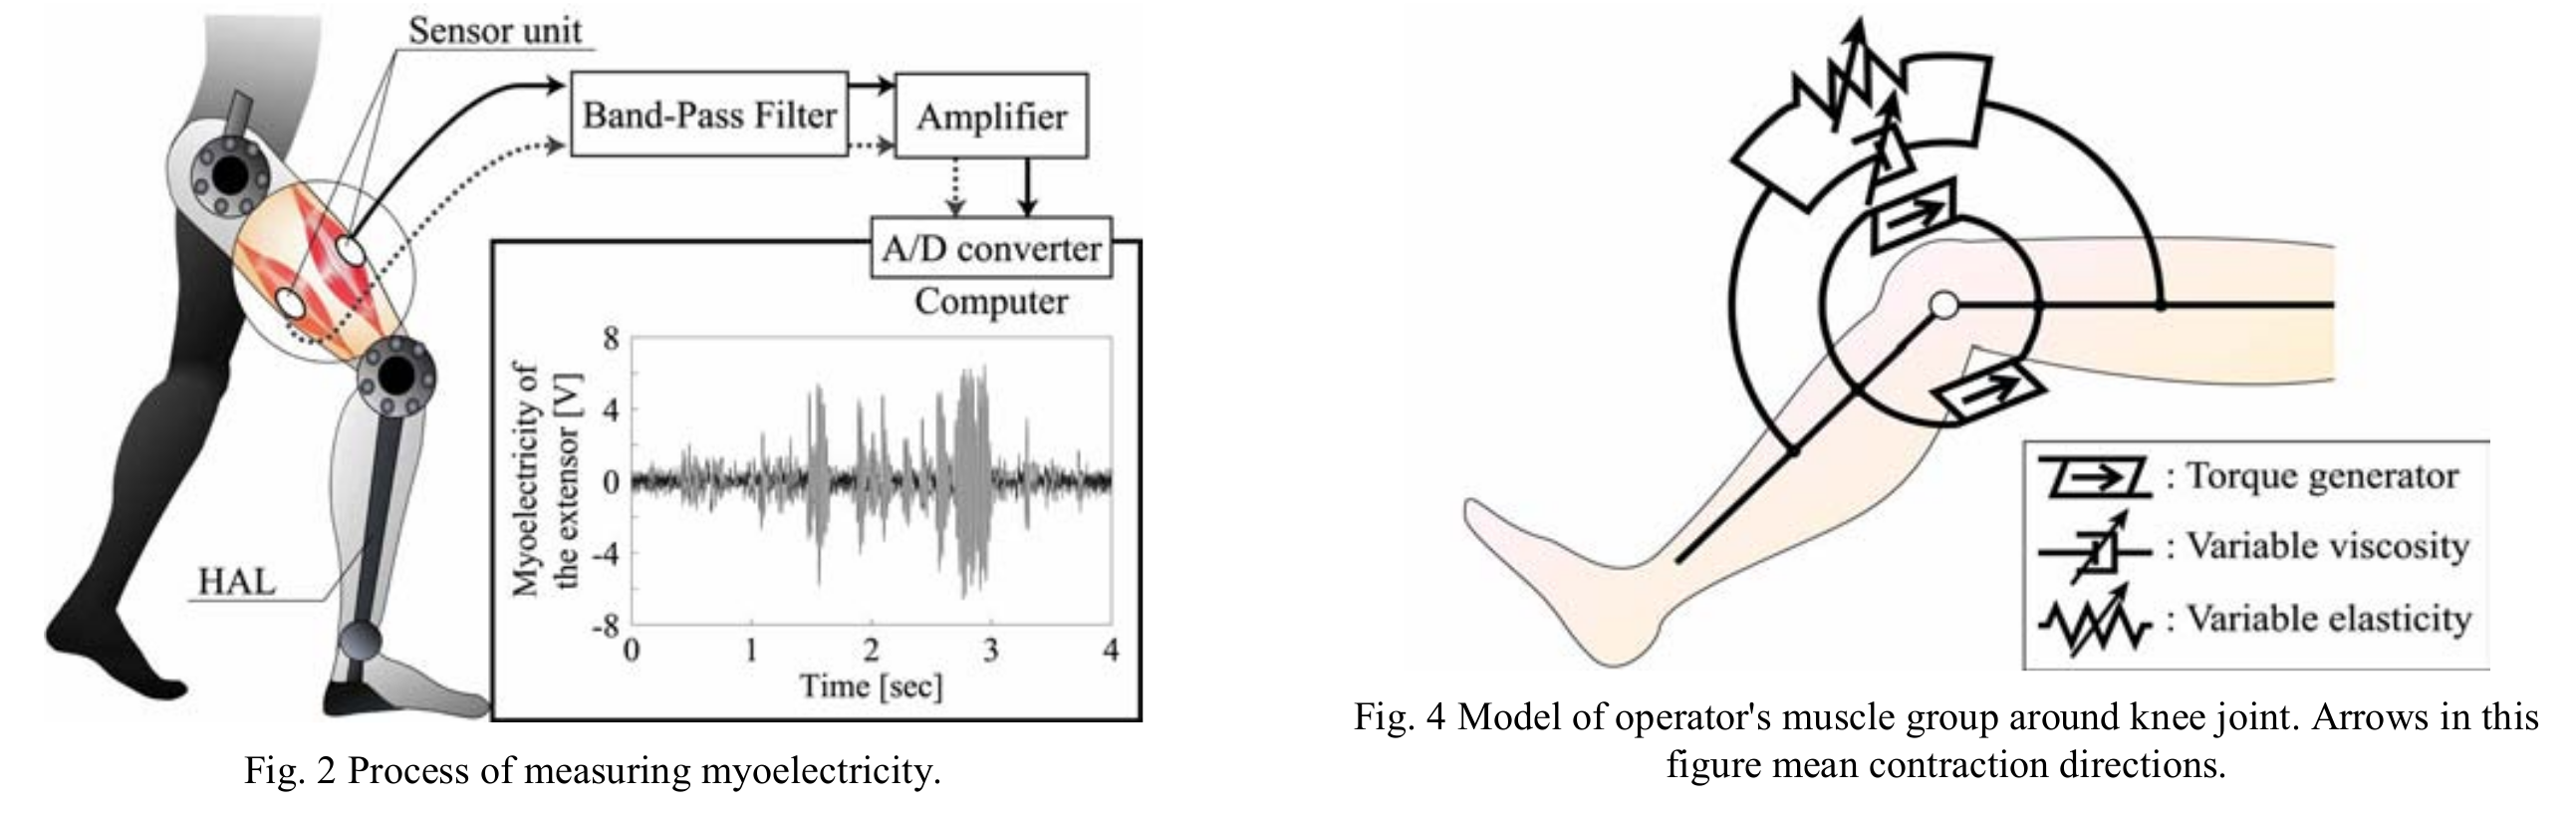
\includegraphics[width=6in]{exos/figs/hal_viscoelastic_control.png}
\end{figure}
%
%

While experiments in \cite{HALmuscleImped2005} only consider leg swing-up and swing-down, a similar control approach in \cite{HALvTorqueImp2002} switches the dynamics based controller to compensate for swing and stance phases in walking gait.  In this case, the gait transitions are detected by thresholding foot sensors and required angular velocity (and acceleration) data are determined by numerically differentiating angular encoders.


\subsection{Assessment and Recommendations}

Compared to sensitivity amplification methods, HAL's use of EMG data allows it to estimate intention without amplifying external disturbances.  While direct sensing of user intention is ideal for noisy, contract-rich environments, sEMG data is extremely difficult to work with due to high filtering and calibration requirements.  A hybrid strategy which uses sensitivity amplification and sEMG data (possibly thresholded) to filter user intention could prove effective.  Additionally, Section~\ref{survey:recommend} mentions new capabilities in nano-fabrication and MEMs technologies that have produced new high-density, wearable sensing arrays. These and similarly advanced sensing technology may facilitate direct measurement of interaction forces (i.e. estimating pressure / force and exoskeleton contact locations), which could potentially filter external disturbances from user generated input to estimate intent.

\nocite{*}
\printbibliography[heading=subbibliography]

The figures in this section were obtained from \cite{HALmuscleImped2005,HALassist2011}.  Materials presented are based on the references above.

\end{refsection}




%%% Local Variables:
%%% mode: latex
%%% TeX-master: "../survey"
%%% End:


\section{XoR}
\label{exo:XoR}
\begin{refsection}[exos/xor.bib]

keywords: model-based control; strength augmentation; hybrid actuation; pneumatic actuation; electric motors;\\

\begin{figure}[ht]
  \centering
  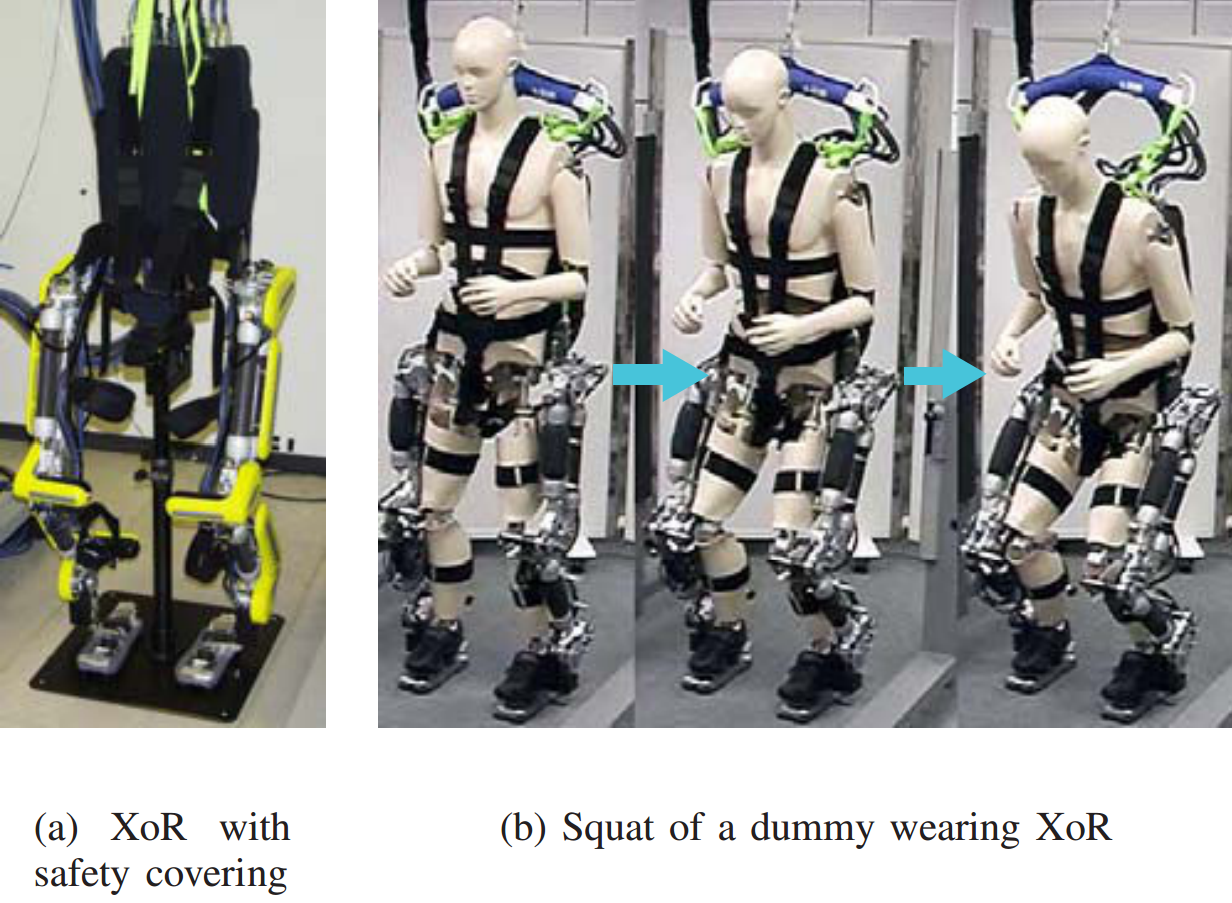
\includegraphics[width=4.0in]{exos/figs/xor.png}
\end{figure}

The XoR is a prototype, light-weight lower-body exoskeleton that uses a hybrid pneumatic-electric drive system that \textbf{reduces weight} while providing \textbf{precise torque control}, \textbf{backdrivability}, and a \textbf{desirable force / velocity} profile.  The exoskeleton is designed to serve in rehabilitation settings to augment operators' strength and assist with postural control for persons with disabilities.

\begin{figure}[ht]
  \centering
  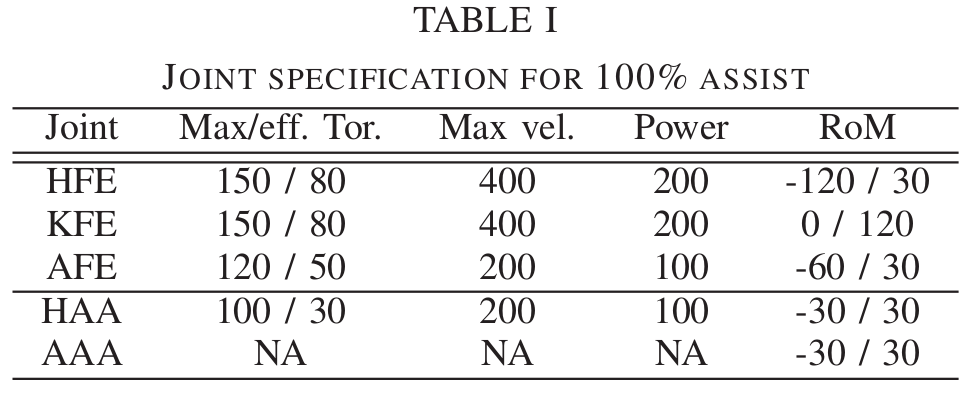
\includegraphics[width=3.5in]{exos/figs/xor_joint_rom.png}
\end{figure}

The XoR weighs 30kg and includes 10 DOF with 6 active joints (flexion / extension of hip, knee, and ankles) and 6 passive (hip abduction/adduction joints, hip rotation, and ankle adduction/abduction).  The active joints are powered by hybrid actuators comprised of an \emph{air muscle} and an electric motor.  The hybrid actuation scheme uses a unilateral air muscle layout to compensate for gravity and bilateral electric motors with relatively small gear ratio (57.5) to serve as the dynamic compensator.

The actuation scheme is complementary in that the electric motors have a quick response time and produce high peak torque for short amounts of time, while air muscles have a delayed response (true of pneumatic systems in general due to the compressibility of air) with better power density and sustained torque.  The hybrid drive system sums the two to develop a desired torque profile that achieves the benefits of both and reduces weight and motor size.  The system offers high torque control with negligable stick-slip and backdrivability.

\begin{figure}[ht]
  \centering
  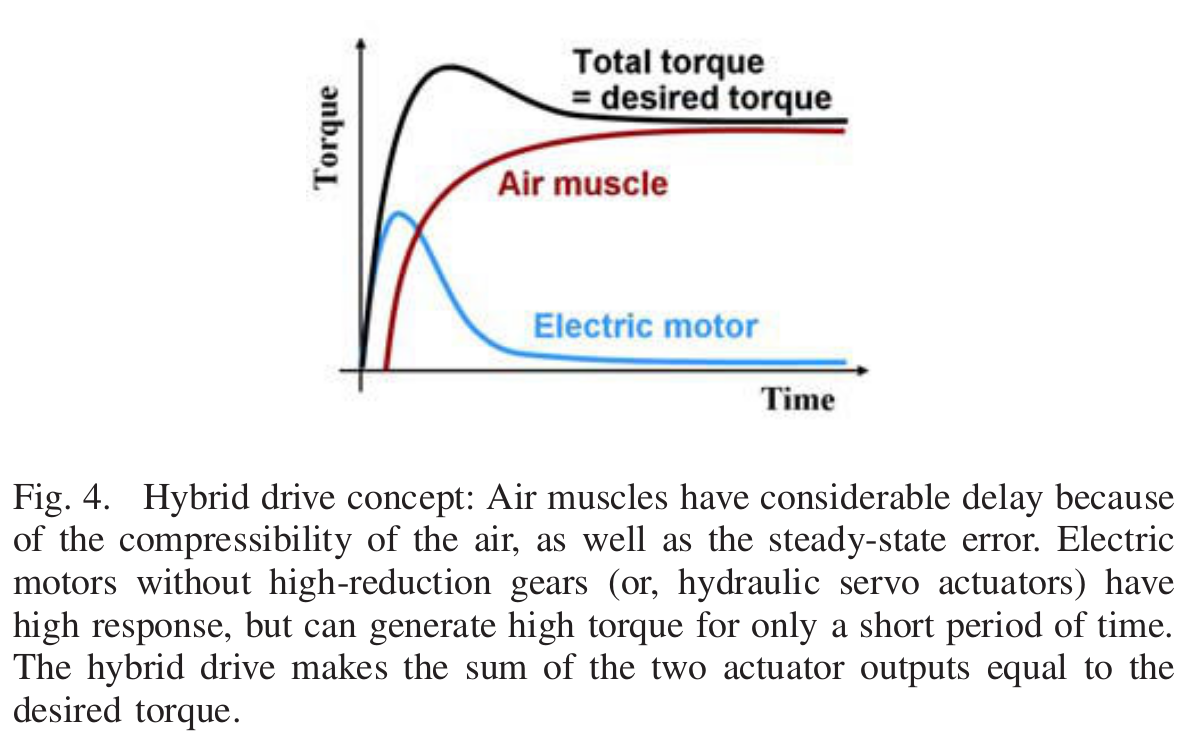
\includegraphics[width=3.5in]{exos/figs/xor_hybrid_drive_torque_time.png}
\end{figure}  

A challenge in using air muscles is that force reduces quadratically as a function of contraction.  For instance, at 30\% contraction, the force produced by FESTO rubber air muscles vanishes.  To address the issue, XoR is strategically places air muscles to generate forces in desired configurations.  

\begin{figure}[ht]
  \centering
  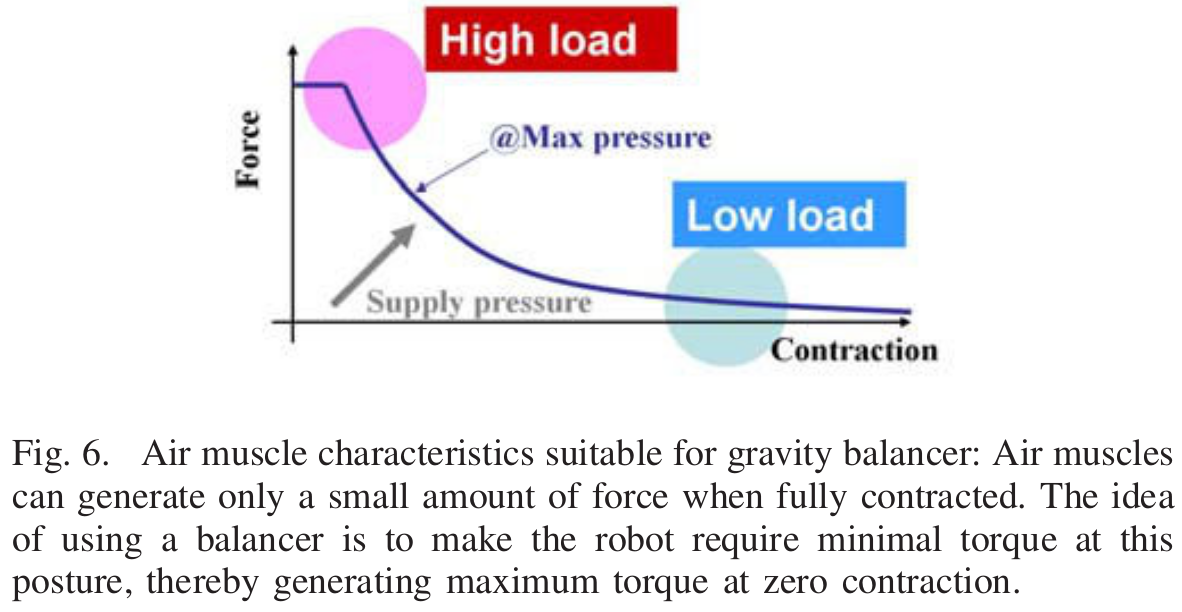
\includegraphics[width=3.5in]{exos/figs/xor_air_muscle_force_vs_contraction.png}
\end{figure}

In implementation, the XoR uses rubber air muscles (MDSP-40) connected to pulleys via tendons and to EP regulators in the backpack (a constant pressure and cam system is being tested to reduce weight required for backpack air valves).  The electric actuator is a geared, 200W brushless DC motor (Maxon EC powermax 30) rated at 4.7 A, which transmits power to joints through a belt and pulley system with a 57.5 gear ratio. the motor's 0.12 Nm output torque provides up to 34.5 Nm (for short duration) at every joint and is backdrivable.  The design yields a relatively high range of motion (up to 120 degrees) with a load capacity 150 Nm.  However, experiments reveal the need for bi-directional pneumatic actuation at hip joints.

For sensing, XoR is equipped with rotary encoders at joints, an IMU in the backpack, load cells in the feet, and is networked to servers capable of providing EMG, NIRS, and EEG data.  A control PC running at 1 KHz, pulse counter, amplifiers, Digital IO are external and so not included in the weight of the unit.  Human operators are outfitted with a goniometer.


\subsubsection{Control}

The XoR control strategy applied in \cite{XoRkinemExtraction2012} has two main components.  First, a proportional-derivative (PD) feedback controller tracks desired joint angles and angular velocities that correspond to the state of the exoskeleton required to assist the human operator.  To obtain this state (specifying the desired joint angles / velocities), the controller simultaneously measures the joint angle trajectories of the human user (goniometer) and of the robot (encoders), and uses canonical correlation analysis (CCA) to extract latent variables in the kinematic relationship between the two.

\begin{figure}[ht]
  \centering
  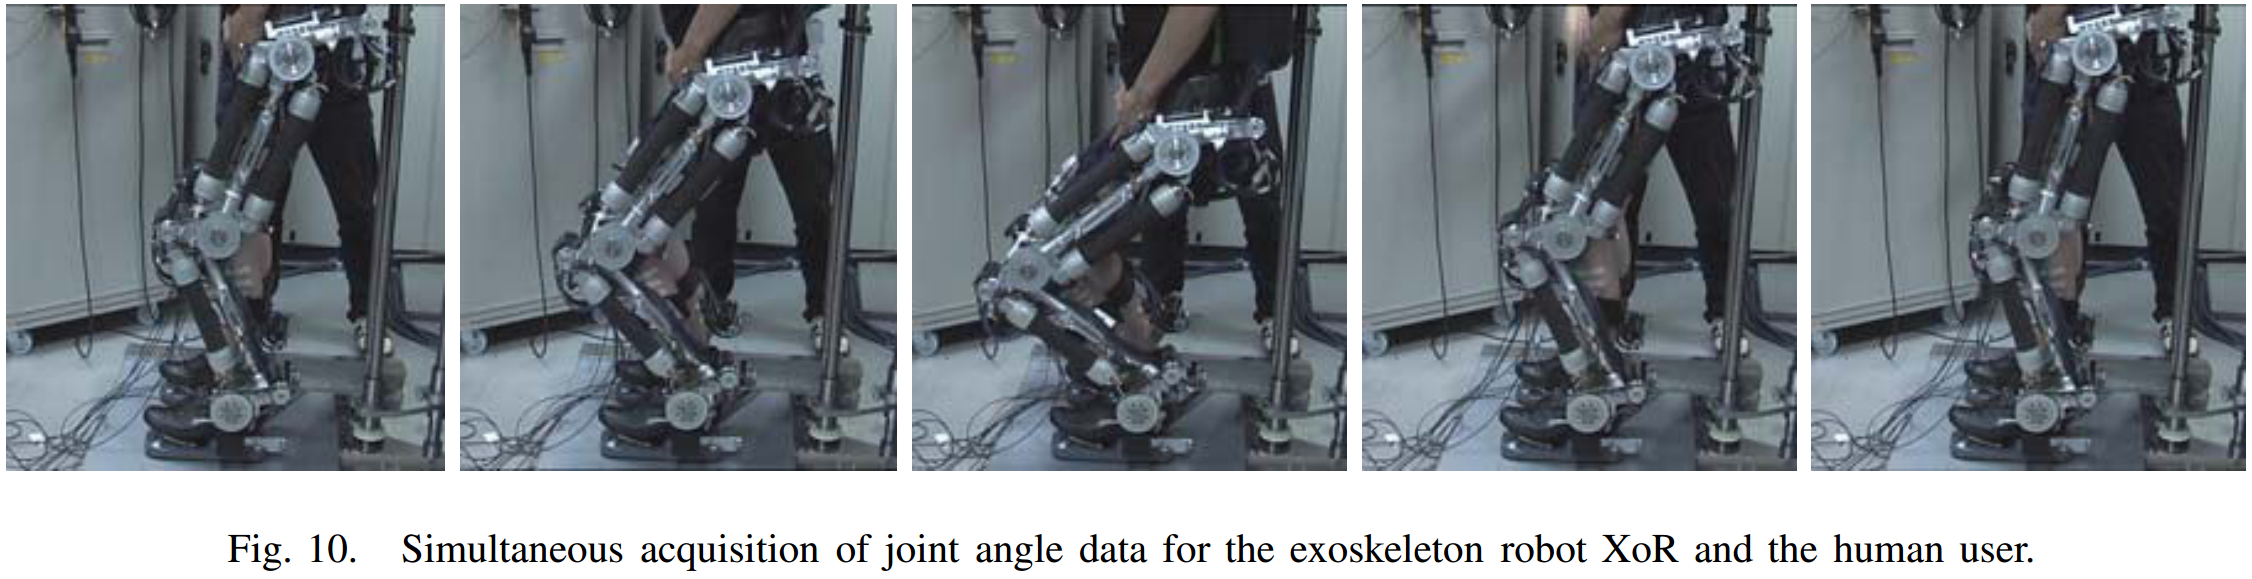
\includegraphics[width=6.0in]{exos/figs/xor_joint_angles.png}
\end{figure}

To avoid relying on high gain feedback, XoR incorporates user intent through EMG data.  The controller rectifies and low pass filters (10 Hz cut-off) data measured in the pilot's quadriceps femoris, tensor fasciae latate, gluteus medius, and tibialis anterior. 
It sets desired joint angles and velocities, ${\bf x} = ({\bf \theta} \dot{\bf \theta})$, from the EMG data, ${\bf u} = (EMG_1 \cdot EMG_n)$, using a linear prediction model, 
\[{\bf x}(k+1) = \mA{\bf x}(k)+\mB{\bf u}(k),\].  
The controller uses the angular measurements required to perform CCA and EMG data to derive the model's $\mA$ and $\mB$ terms.  The predicted state from EMG model provides the desired input to yet another PD controller: 
\[\tau_i = K_p (\theta_i^d - \theta_i) + K_d (\dot\theta_i^d - \dot \theta_i),\] 
with gains of $K_p = 1000$ and $K_d = 100$.

In hip tracking experiments, the team found EMG data to be helpful.  When using EMG signals, XoR achieved a mean squared error of $1.8E^{-3}$.  Without the EMG data, the mean squared error increased to $2.1$.  Additional experiments confirm the air muscles can effectively perform gravity compensation when used in conjunction with electric actuators (to correct for torque errors induced by inaccuracies in the model mapping position to toque in air muscles).


\subsection{Assessment and Recommendations}

The XoR prototype uses a promising hybrid actuation scheme to achieve both fast peak torque response and higher sustained torque while remaining lightweight.  They track human motion with feedback from a goniometer and feedforward control provided by EMG data.  These human intention / sensing modalities are both difficult to implement due to noise and calibration issues.  However, capturing the user intent is important, especially in the presence of external disturbances.  If the sensory system were improved (e.g, wearable ``robot skin'' sensing arrays), this exoskeleton design could be highly effective. 

\nocite{*}
\printbibliography[heading=subbibliography]

The figures in this section were obtained from \cite{xorDesign2011,XoRkinemExtraction2012}. Materials presented are based on the references above.

\end{refsection}

% % Created 2015-09-15 Tue 11:46
% \documentclass[11pt]{article}
% \usepackage[utf8]{inputenc}
% \usepackage[T1]{fontenc}
% \usepackage{fixltx2e}
% \usepackage{graphicx}
% \usepackage{longtable}
% \usepackage{float}
% \usepackage{wrapfig}
% \usepackage{rotating}
% \usepackage[normalem]{ulem}
% \usepackage{amsmath}
% \usepackage{textcomp}
% \usepackage{marvosym}
% \usepackage{wasysym}
% \usepackage{amssymb}
% \usepackage{hyperref}
% \usepackage{color}
% \usepackage{soul}
% \tolerance=1000
% \usepackage[margin=1in]{geometry}

% \newcommand{\hilight}[1]{\colorbox{yellow}{#1}}


%\begin{document}
\section{Body Extender}
\label{bodyExtender}
\begin{refsection}[exos/bodyExt.bib]

The Body Extender is one of the few existing full-body exoskeletons.  The Body Extender's main objective is to increase the forceful interaction capabilities, specifically the heavy load handling capabilities, of an operator in difficult and unknown environments.  The overall suit is composed of four robotic limbs with kinematics designed to be anthropomorphically similar.  The suit contains twenty-two independently actuated degrees of freedom.  Note that the Body Extender is the only fully actuated suit included in this report.  The fully actuated design of the suit was chosen based on the fact that handling, or rather manipulating heavy objects requires forces and torques that far exceed human capabilities.  Note also that having many actuated degrees of freedom means that fully actuated suits will be very heavy, and thus will require specialized controllers.

As a primary objective, the Body Extender aims to allow operators to use the hardware with minimal training.  Thus, the system is designed so as not to require substantial modifications to human motor habits.  The effective mass distribution of the suit, of special consideration in these heavy systems, is designed to be similar to that of an unloaded operator.  Like most other strength augmentation exoskeletons, the Body Extender is intended to minimize resistive forces between the operator and suit, even when the suit is not loaded externally. 

A picture of the Body Extender exoskeleton and its five main components, four limbs and a torso, is shown in Figure \ref{fig:bodyExt}.
\begin{figure}[thpb]
\centering
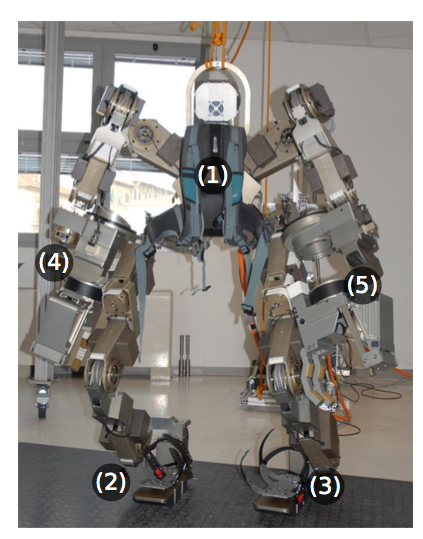
\includegraphics[width=3.in]{exos/figs/bodyExt/bodyExt}
  \caption{The Body Extender.}
%  \vspace{-0.2in}
 \label{fig:bodyExt}   
 \end{figure}
 

\subsection{Actuator Specifications}
 
 Except for forearm pronosupination, each of the actuators in the Body Extender suit are driven by a linear actuator that is composed of an electrical motor, incremental encoder, ball screw, and angular contact ball bearings.  The motors are frameless DC torque controlled motors.  The {\bf peak torque of the motors is 7 Nm, with a maximum continuous torque of 6 Nm}.  Each motor weighs 1.4 kg.  The {\bf linear actuator assembly is able to supply 8000 N with a total weight of 2.4 kg}.
 
 Joints that have a small range of motion and low torque requirements use linear actuators in straightforward lever mechanism configurations.  For degrees of freedom which require relatively large ranges of motion as well as torque, a motion conversion system transforms the linear actuator motion into rotational motion.  The motion conversion unit consists of a pantograph, two metallic tendons, and an output pulley connected to the output link.  A CAD drawing of the motion conversion unit is shown in Figure \ref{fig:motionConv}. 
 \begin{figure}[thpb]
\centering
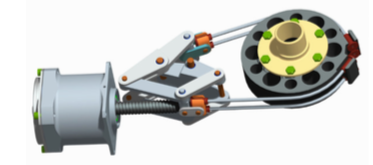
\includegraphics[width=3.in]{exos/figs/bodyExt/motionConv}
  \caption{CAD view of the internal components of the actuation module.}
%  \vspace{-0.2in}
 \label{fig:motionConv}   
 \end{figure}
 There are two configurations of the motion conversion unit.  The first has a {\bf maximum continuous output of 500 Nm and the second a maximum continuous output of 270 Nm}.  The two units weigh 6 kg and 5 kg respectively, and have {\bf mechanical efficiency of about 85\%}.  {\bf The speed of the actuators is approximately 60 deg/s}.
 
 
 \subsection{Exoskeleton Specifications}
 
 The Body Extender's twenty-two actuated degrees of freedom include two arms, two legs, and a torso or central backpack unit.   The arms have a servo-amplified degree of freedom for grasping heavy objects.  Grasping forces are achieved using a force sensing trigger mechanism; the force is proportional to the force applied to the trigger.
 
 The suit contains twenty-two incremental encoders that measure angular displacement of each of the electric motors.  There are also {\bf five six-axis force/torque sensors mounted at the five connecting points between the user and the device; two at the hands, two at the feet, and one on the trunk.}  These sensors directly measure the forces and torques between the user and the suit.  There are additionally two single axis force sensors integrated into the grippers that measure the force applied by the operator on the ``gripper triggers," as well as {\bf a three axis accelerometer integrated into the backpack unit which estimates the trunk orientation}.  Lastly, \textbf{accelerometers are distributed throughout the system} to monitor link dynamics, supporting overall equilibrium and internal stability during manipulation tasks.   
 
{\bf The control software is distributed between a central processing unit and sixteen local units located throughout the system}.  The communication between processing units is handled using a high-speed field bus.
 
{\bf The system is powered using thirteen batteries in series, which provide a nominal voltage of 78 V}.  When the system is run in stand-alone mode, the batteries can provide eight hours of continuous work.
 
 
 \subsection{Control Specifications}
 
 The body extender control algorithm centers around a {\bf feedback linearization policy} that depends on measuring the force between the operator and suit, knowing the contact state of the suit and environment, decoupling the control of each of the limbs for each other, and having each limb be fully actuated.  The dynamics for each of the Body Extender limbs are written in standard form as  
\begin{equation}
\mB_i(q) \ddot{q} + \mC_i(q,\dot{q})\dot{q} + \mG_i(q) = {\bf \tau} + \mJ^T_{iu}{\bf F_s} + \mJ^T_{ia}{\bf F_a},
\end{equation}
where $i$ is an integer corresponding to a different limb, ${\bf \tau}$ represents the actuator torques, ${\bf F_s}$ the measured forces between the operator and suit, and ${\bf F_a}$ the unmeasured contact forces on the suit.  The $\mB_i$, $\mC_i$, and $\mG_i$ terms represent the limb inertia, Coriolis and centrifugal, and gravitational torques.  

The authors in \cite{body_control_2012} use a decoupling strategy in their controllers which enables the individual limbs in the Body Extender to be somewhat decoupled from each other.  They claim that they accomplish this using the following model:
\begin{equation}
\mB_i(q) \ddot{q} + \mC_i(q,\dot{q})\dot{q} + \mG_{iT}(q) = {\bf \tau} + \mJ^T_{iu}F_s + \mJ^T_{ia}F_a - \mB_{iT}{q}\dot{V}_T - \mC_{iT}(q,\dot{q}){\bf V_T},
\end{equation}
where, ${\bf V_T}$ is the trunk velocity, $\mG_{iT}$ the gravitational effect of the trunk on the limb, $\mB_{iT}$ the inertia of the trunk acting on the limb, and $\mC_{iT}$ the trunk Coriolis and centrifugal term.  Note that ${\bf V_T}$ and $\dot{{\bf V}}_{\bf T}$ are directly measured through the accelerometer and gyroscope in the trunk.

The feedback linearizing controller in \cite{} operates under two fundamental assumptions and only appears to relate directly to the case of a single manipulator arm.  The first assumption of the controller is that the mass and inertial properties of an object being manipulated are estimated online.  The second is that the forces measured between the operator and suit can be modeled as
\begin{equation}
\vF_s = \mM_p \dot{\vV}_e + \vG_p,
\label{eq:forceEq}
\end{equation}
where $\mM_p$ is an effective mass of the end effector, $\dot{\vV}_e$ is the acceleration of the end effector, and $\mG_p$ is an effective gravitational term.  Note that the gravitational term is zero if the arm is not holding an external load.  The importance of these two assumptions will be more clear after the analytical forms of the feedback linearizing controllers are introduced. 

The dynamics of the arm when not manipulating a load are
\begin{equation}
\mB(\vq) \ddot{\vq} + \mC(\vq,\dot{\vq})\dot{\vq} + \mG(\vq) = {\bf \tau}. \notag
\end{equation} 
The feedback linearizing controller for this case has the form
\begin{equation}
{\bf \tau} = \mB(\vq)(\ddot{\vq}_d + K_v \dot{\tilde{\vq}} + K_p \tilde{\vq}) + \mC(\vq,\dot{\vq})\dot{\vq} + \mG(\vq), \notag
\end{equation}
where $\tilde{\vq} = \vq_d - \vq$.  The details are unclear in \cite{body_control_2012}, but it appears that the authors either propose using predefined trajectories to define $\ddot{\vq}_d$, $\dot{\vq}_d$, and $\vq_d$, or use the assumption in \eqref{eq:forceEq} to determine these values.  
%\begin{equation}
%\vF_s = \mM_p \dot{V}_e
%\label{eq:assump1}
%\end{equation}
Equation \ref{eq:forceEq} relates the measured force to the derivative of the end effector velocity $\dot{\vV}_e$.  This end effector velocity can then be related to the desired joint velocities using the analytical Jacobian transformation \[ \ddot{\vq}_d = \mJ(\vq)^{-1}(\dot{V}_e - \dot{J}(\vq,\dot{\vq})\dot{\vq}).\]  The values for $\dot{\vq}_d$ and $\vq_d$ can then be found through integration.  It is not clear the how authors explicitly decouple the human dynamics from the robot in this case.

In the case where the exoskeleton arm is manipulating a load, the feedback linearizing controller has the augmented form
\begin{equation}
{\bf \tau} = \mB(\vq)(\ddot{\vq}_d + K_v \dot{\tilde{\vq}} + K_p \tilde{\vq}) + \mC(\vq,\dot{\vq})\dot{\vq} + \mG(\vq) -\mJ^T(\vq) \vF_s -\mJ^T(\vq)\vF_a. \notag
\end{equation}
The main difference in this case is that the controller here explicitly compensates for the measured human-robot interaction force $\vF_s$, and the controller includes the un-sensed forces $\vF_a$ which arise from the object being manipulated.  The object interaction forces thus need to be estimated.  The ability to estimate these forces is the first fundamental assumption on which the Body Extender's control scheme relies.  Because the point at which the manipulator arm and object are connected is assumed to be well known, and the arm is instrumented with inertial sensors, estimating the interaction forces of the manipulated object is be assumed to be equivalent to estimating its inertial properties.  As outlined in \cite{body_control_2012}, this is accomplished using a standard regressor which uses the input and output of the feedback linearizing controller as the basis for the regression.  The details of this process are left to \cite{body_control_2012}.

 
\subsection{Assessment and Recommendations}

The Body Extender suit is one of the only full-body exoskeletons available today, and as such is a somewhat remarkable system. In terms of how the Body Extender system is designed and how it is controlled, the suit may be limited. Clearly, for the task of handling heavy objects a fully actuated suit may be the best option, but, generally speaking, this seems almost like an over engineered solution.  The Body Extender is a heavy, overly clunky suit.  This suit may be alright for quasi-static operations, but it is unlikely that it will be useful for more than pick and place type operations.  Again, seeing as this is basically what it was designed for, that seems alright.

In terms of the controllers highlighted in \cite{body_control_2012}, there are some good ideas.  For example, using a regressor to estimate unknown external forces may be an idea which is directly applicable to the TALOS project.  In the case of the Body Extender this regression is dependent on knowing at the location of the external force  relative to the suit, but the idea in general is interesting.  The idea of using the measured forces to generate desired trajectories around which a stabilizing controller is designed also appears to be a relatively good idea.  Note that, like any of the model-based control approaches outlined in the exoskeleton literature, or robotics literature for that matter, the feedback linearizing controller in this work is dependent on knowing the model of the robot hardware.  

In terms of the control of the overall suit, it was difficult to find any control papers about the Body Extender that covered anything other than upper-body single-arm control of a manipulated object.  The strategy of decoupling the individual limbs from each other, seems somewhat feasible, but is not the best way to approach coordinated limb control.  It was difficult to find literature documenting the specifics of lower-limb control for the Body Extender.  Presumably a similar strategy to that discussed here, with the addition of gravity compensation for the suit, is used.

 The mechanical specifications as well as figures related to mechanical design for the Body Extender system discussed in this section are based on and taken from \cite{body_design_2011}.  The discussion of the control system is based on work presented in \cite{body_control_2012}.

\printbibliography[heading=subbibliography]

\end{refsection}
  
% \end{document}


% S. Marcheschi, F. Salsedo, M. Fontana, and M. Bergamasco, Body Extender: Whole body exoskeleton for human power augmentation, in Proc. IEEE Int. Conf. Robotics Automation, 2011, pp. 611?616.


% G.P. Rosati Papini, and C.A. Avizzano, "Transparent Force Control for Body Extender," 2012 IEEE RO-MAN: The 21st IEEE International Symposium on Robot and Human Interactive Communication, 2012, pp. 138-143.




%%% Local Variables:
%%% mode: latex
%%% TeX-master: "../survey"
%%% End:


% % Created 2015-09-15 Tue 11:46
% \documentclass[11pt]{article}
% \usepackage[utf8]{inputenc}
% \usepackage[T1]{fontenc}
% \usepackage{fixltx2e}
% \usepackage{graphicx}
% \usepackage{longtable}
% \usepackage{float}
% \usepackage{wrapfig}
% \usepackage{rotating}
% \usepackage[normalem]{ulem}
% \usepackage{amsmath}
% \usepackage{textcomp}
% \usepackage{marvosym}
% \usepackage{wasysym}
% \usepackage{amssymb}
% \usepackage{hyperref}
% \usepackage{color}
% \usepackage{soul}
% \tolerance=1000
% \usepackage[margin=1in]{geometry}

% \newcommand{\hilight}[1]{\colorbox{yellow}{#1}}

% %\author{Alex Ansari}
% %\date{}
% %\title{TALOS}
% %\hypersetup{
% %  pdfkeywords={},
% %  pdfsubject={},
% %  pdfcreator={Emacs 24.3.1 (Org mode 8.2.10)}}


% \begin{document}
\section{Hydraulic Lower Extremity Exoskeleton}
\label{dualMode}
\begin{refsection}[exos/dualMod.bib]

The Hydraulic Lower Extremity Exoskeleton suit was originally developed for military uses, specifically to allow operators to perform motions without incurring muscle fatigue.  The exoskeleton uses a new {\bf virtual joint torque control} approach, which has been shown to be effective for controlling human robot interaction in situations where the connections between the users and hardware system are relatively unknown or can dramatically change as a function of time.

Additionally, the main hardware design principle is focused on developing a suit that can augment user power and yet move fast when necessary.  The design team selected hydraulic actuators because the weight of electric actuators on leg joints would make the system difficult to move quickly.  Hydraulic actuators have high power density relative to weight and size and generally provide very high force outputs and low impedance.  As a trade-off, hydraulics have reduced accuracy in terms of force control and it is difficult to model their nonlinear characteristics.  

A picture of the Hydraulic Lower Extremity Exoskeleton is presented in Figure \ref{fig:exoSuit}.
\begin{figure}[thpb]
\centering
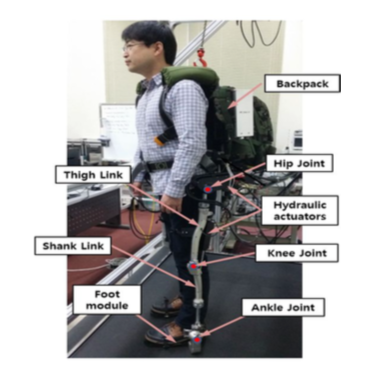
\includegraphics[width=3.in]{exos/figs/hydLowerExrem/exoSuit}
  \caption{Exoskeleton robot system.}
%  \vspace{-0.2in}
 \label{fig:exoSuit}   
 \end{figure} 
 

\subsection{Actuator specifications}

The Hydraulic Lower Extremity Exoskeleton's actuators were designed based on human walking data obtained at 4km/h with a 45 kg load.  Based on this data, the hydraulic capacity system was designed to provide 2050psi and 8lpm.  The individual actuators were designed to be double acting at the hip and knee flexion/extension joints. They provide a {\bf hip maximum thrust of 4 kN} and {\bf knee maximum thrust of 4 kN}.  Each joint joint includes three-way servo valves (M 200, Star-Hydraulic) to control rate and direction of bi-directionality, and bypass valves to connect the pump path to tank path for fast, energy-efficient motion during swing phases.   

The hydraulic system for each joint is shown in Figure \ref{fig:hydraulicSys}.
A picture of the Hydraulic Lower Extremity Exoskeleton is presented in Figure \ref{fig:exoSuit}.
\begin{figure}[thpb]
\centering
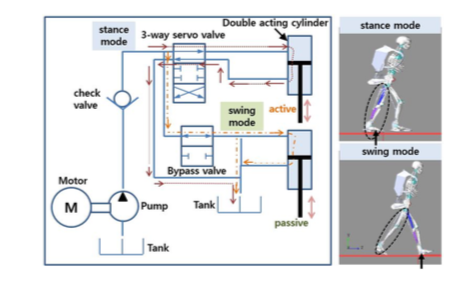
\includegraphics[width=3.in]{exos/figs/hydLowerExrem/hydraulicSys}
  \caption{Dual-mode control}
%  \vspace{-0.2in}
 \label{fig:hydraulicSys}   
 \end{figure} 


%\begin{figure}[thpb]
%\centering
%\includegraphics[width=3.in]{figs/seaAssm}
%  \caption{}
%  \vspace{-0.2in}
% \label{fig:IHMCSEA}   
% \end{figure}
 

 
 \subsection{Exoskeleton Specifications}
 
 The Hydraulic Lower Extremity Exoskeleton includes four actively controlled joints in the sagittal plane, with powered knee and hip flexion/extension.  The eight passive joints include one ab/adduction DOF for each hip and 3 DOF for each ankle.
 
 The hydraulic system is composed of the four actuators and a hydraulic power unit, consisting of a pump, motor, temperature sensor, and various valves.
 
 On-board sensors measure \textbf{joint angles}, \textbf{actuator forces}, and \textbf{ground reaction forces}.  Three \textbf{absolute angular encoders} are incorporated at the hip, knee, and ankle pitch joints.  In-line \textbf{load cells} are incorporated in each cylinder tube to measure actuator forces, and four single axis load cells are included in foot sensors to be used for gait phase detection.
 
 \subsection{Control Specifications}
 
 \begin{figure}[thpb]
\centering
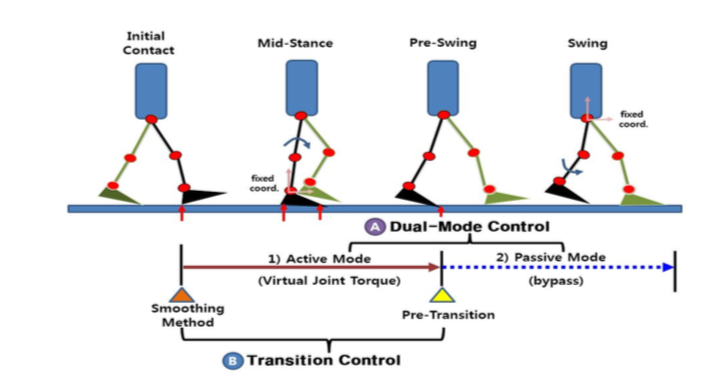
\includegraphics[width=5.in]{exos/figs/hydLowerExrem/dualModeDia}
  \caption{Locomotion control strategy during gait : Smoothing method ! Active mode ! Pre-transition method ! Passive mode}
%  \vspace{-0.2in}
 \label{fig:dualModeDia}   
 \end{figure}
The control design principle for the Hydraulic Lower Extremity Exoskeleton is based on the concept that, for walking gaits, the {\bf stance and swing controllers should be considered separately}.  To this end, the control designers developed an active-passive control method called {\bf Dual-Mode Control}.  Active control is used during stance phases whereas the passive control is used to quickly and freely control the system's legs during swing phases.  Additionally, to handle the inherently discontinuous jumps in the command signals that occur in this dual mode abstraction, a smoothing method is used in conjunction with a pre-transition method that solves for the swing delay due to internal cylinder pressure.  A diagram which highlights the different modes in this control strategy is in Figure \ref{fig:dualModeDia}.   

Various components of the dual-mode control strategy, at the hardware level, are presented in Figure \ref{fig:suitDia}.  
  \begin{figure}[thpb]
\centering
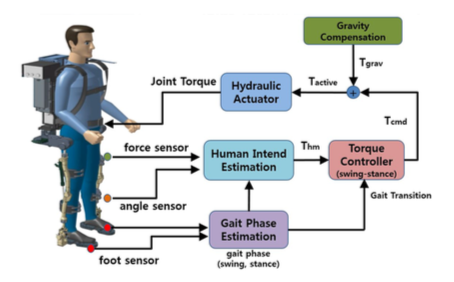
\includegraphics[width=3.in]{exos/figs/hydLowerExrem/suitDia}
  \caption{Overall control block diagram.}
%  \vspace{-0.2in}
 \label{fig:suitDia}   
 \end{figure}
This figure contains a {\bf gait phase estimation block}, which uses the foot sensors to estimate the stance mode of the system, a {\bf human intention block}, which uses angular encoders and joint force sensors to estimate the motion of the operator, a {\bf torque controller}, and a {\bf gravity compensation} block.  Note that these various components of the control system are used to support the general assumption of the dual mode controller, i.e., 
 \begin{figure}[thpb]
\centering
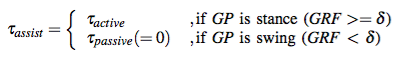
\includegraphics[width=3.in]{exos/figs/hydLowerExrem/torAssist}
%  \caption{Simplified virtual joint torque control block diagram}
%  \vspace{-0.2in}
% \label{fig:suitDia}   
 \end{figure}
 %
 \noindent
where, $GP$ is the gait phase, $GRF$ is the ground reaction force, and $\delta$ is a threshold value.  This equation explicitly states that an active torque will be applied for each leg during stance and that the legs are passive in their respective swing phases.

Like other controllers presented in this report, the dual mode control method in this section uses the fundamental assumption that it is difficult to measure the interaction forces between the user and hardware system directly as a primary design principle.  To this end, the human-robot interaction force is assumed to be completely represented in terms of the joint torque applied by the operator in the hardware. 

To calculate the active torque applied to the joints during the active mode control, the robot dynamics are considered independently from the operator, namely,
\begin{equation}
\vT_a = \mM(\vq)\ddot{\vq} + \mC(\vq,\dot{\vq})\dot{\vq}+\mG(\vq),
\label{dynamics}
\end{equation}   
where $\vT_a$ is the joint torque applied by the actuators, $\mM(\vq)$ is the inertia matrix, $\mC(\vq,\dot{\vq})$ is the centripetal and Coriolis matrix, and $\mG(\vq)$ is the gravitational torques. note that this equation neglects friction as well as other actuation dynamics.

Using the force sensors on the hydraulic actuators, the {\bf human-robot interaction torques} can be approximated as
\begin{equation}
\hat{\vT}_{hm} = \mM_n(\vq)\ddot{\vq} + \mC_n(\vq,\dot{\vq})\dot{\vq} + \mG_n(\vq) - \hat{\vT}_a, \notag
\end{equation}
where $\mM_n$, $\mC_n$, and $\mG_n$ are the nominal models of the true inertia, centripetal, and gravitational parameters and $\hat{\vT}_a$ represents the measured actuator torques.  The $\mM_n(\vq)\ddot{\vq} + \mC_n(\vq,\dot{\vq})\dot{\vq} + \mG_n(\vq) $ portion of $\hat{\vT}_{hr}$ represents the inverse dynamics component of the closed-loop control system.  The overall joint torque controller, which combines compensation for operator intent as well as balancing of the suit under a gravitational load, is then written \[ {\bf\tau}_\text{active} = K(s) \hat{\vT}_{hm} + \mG_n(\vq),\] where $K(s) = K_p +s K_d,$ i.e., there is closed-loop PD control law operating on the error between the predicted robot dynamics and the measured joint torques.  The block diagram for the active mode controller is shown in Figure \ref{fig:blockDia}. 
 \begin{figure}[thpb]
\centering
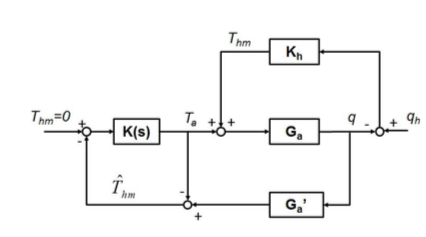
\includegraphics[width=3.in]{exos/figs/hydLowerExrem/blockDia}
  \caption{Simplified virtual joint torque control block diagram.}
%  \vspace{-0.2in}
 \label{fig:blockDia}   
 \end{figure}
 Note that $\mG_a$ represents the dynamics of the the system and $\mG_a'$ the inverse dynamics model in Figure \ref{fig:blockDia}.

 In the passive mode, which occurs during the swing phase, the leg of the human-robot system moves quickly and freely under using the passive inertial forces of the overall system.  This is accomplished using bypass valves that connect the pump and tank paths to achieve mechanical back-drivability.  The foot sensors trigger the bypass valves and to initiate the pass control mode.

The Hydraulic Lower Extremity Exoskeleton uses a novel scheme to manage transitions between the active and passive control modes.  In particular, the controller applies an explicit smoothing method to address discontinuities in the command torque at phase transitions.  The implementation proposed uses an exponential weighting function of the form
 \begin{figure}[thpb]
\centering
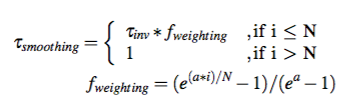
\includegraphics[width=3.in]{exos/figs/hydLowerExrem/weightingForm}
%  \caption{Simplified virtual joint torque control block diagram.}
%  \vspace{-0.2in}
% \label{fig:suitDia}   
 \end{figure}
 
 \noindent
 where ${\bf\tau}_\text{inv}$ is the inverse dynamics torque associated with the robot model, $f_\text{weighting}$ is the weighting function, $a$ is a sensitivity factor, and $N$ describes the duration of the transition period.  The transition duration period as well as sensitivity factor appear to be hand tuned parameters. 

In addition to phase transition smoothing, a pre-transition control method is applied at the end of the stance phase prior to the passive swing phase in order to affect smooth phase transitioning.  The pre-transition control works by measuring the ground reaction force and setting a minimum threshold value.  When the GRF drops below the threshold the system enters a passive swing control mode, i.e., the bypass valve at the actuators are opened.  The objective of this method is to reduce the phase transition delay due to residual pressure in the foot sensors. 


 
 \subsection{Assessment and Recommendations}
 
The design of the Hydraulic Lower Extremity Exoskeleton has a lot going for it.  The best part of this hardware as well as control design is the fact that the creators of it are doing something relatively straightforward.  The actuators are composed of what appears to be off-the-shelf components, and the addition of bypass valves to take advantage of passive dynamics during walking to produce more energy conscious behaviors is a good idea.    

One potential drawback of this hardware is the power system.  The documentation in \cite{} was sparse with respect to the exact specifications of the motor and energy storage device which powers the hydraulic system.

The control system for this hardware followed a relatively straight-forward design, effectively creating a ``get out of the way design" using the torque sensed at the joints only.  In the short-term, this type of policy seems to be a good strategy.  The other highlight of the outlined control policy was the smoothing function which was used during phase transitions in the walking gait cycle.  A similar type of smoothing will most likely be beneficial in terms of operator experience for a varity of different operational modes in which different phase transitions occur, e.g., running, jumping, etc.
 
The figures as well as hardware and control specifications in this section are taken from \cite{dual_mode_2015}.
 
\printbibliography[heading=subbibliography]

\end{refsection}

 
 % \end{document}

 
 % Hongchul Kim and Changhoon Seo and Young June Shin and Jung Kim and Youn Sik Kang, "Locomotion Control Strategy of Hydraulic Lower Extremity Exoskeleton Robot," IEEE International Conference on Advanced Intelligent Mechatronics, 2015, pp. 577-582.
 
 
 

%%% Local Variables:
%%% mode: latex
%%% TeX-master: "../survey"
%%% End:


% % Created 2015-09-15 Tue 11:46
% \documentclass[11pt]{article}
% \usepackage[utf8]{inputenc}
% \usepackage[T1]{fontenc}
% \usepackage{fixltx2e}
% \usepackage{graphicx}
% \usepackage{longtable}
% \usepackage{float}
% \usepackage{wrapfig}
% \usepackage{rotating}
% \usepackage[normalem]{ulem}
% \usepackage{amsmath}
% \usepackage{textcomp}
% \usepackage{marvosym}
% \usepackage{wasysym}
% \usepackage{amssymb}
% \usepackage{hyperref}
% \usepackage{color}
% \usepackage{soul}
% \tolerance=1000
% \usepackage[margin=1in]{geometry}

% \newcommand{\hilight}[1]{\colorbox{yellow}{#1}}

% %\author{Alex Ansari}
% %\date{}
% %\title{TALOS}
% %\hypersetup{
% %  pdfkeywords={},
% %  pdfsubject={},
% %  pdfcreator={Emacs 24.3.1 (Org mode 8.2.10)}}


% \begin{document}
\section{IHMC Mobility Assist Exoskeleton (MAE)}
Although the IHMC MAE was primarily designed as a disabled assist exoskeleton, the device is also provides a ``performance enhancement" control mode, which is within the scope of this document.  The main design principle highlighted in the IHMC MAE hardware (a recurring theme throughout exoskeleton literature) is that directly measuring user intent can be difficult for a number of reasons.  The IHMC designers resolve the issue using a new control and feedback system, which for the IHMC MAE, is primarily based on a unique actuation scheme. 

The IHMC MAE uses novel series elastic actuators (SEAs) in their hardware design mostly because they offer the ability to perform high-fidelity impedance control.  In series elastic actuators, a compliant element is placed in series after the output a motor's drive mechanism. The measured compression of the compliant element is used to calculate the force, or torque, acting on the output of the actuator.  { \bf Series elastic actuators} are generally viewed as a good way to provide {\bf accurate force feedback} information and to provide a {\bf low mechanical impedance}.  The major disadvantage of SEAs is that they have a relatively low bandwidth at high forces, as the compliant element needs time to compress before a force can be sensed and thus inherently include a delay between the time a force is applied and when the control system can react.

\subsection{Actuator specifications}

The IHMC actuators are designed based on data collected from clinical gait analysis.  Specifically, the actuators at the hip and knee were designed to be able to provide 40Nm of peak torque during the stance phase of the walking gait cycle.  The rotary SEA is composed of a Moog BN34-25EU-02 brushless DC motor with a 1:100 harmonic drive (SHD-20).  
 
The spring mechanism, which sits between the gearbox and joint output, is shown in Figure \ref{fig:IHMCSEA}.  The mechanism uses linear die springs and an angular encoder to measure the joint torque output.  The choice of linear die spring was based on the spring's predictable force to displacement function as well as favorable energy storage to weight characteristics.  
\begin{figure}[thpb]
\centering
\includegraphics[width=3.in]{exos/figs/ihmc/seaAssm}
  \caption{}
  \vspace{-0.2in}
 \label{fig:IHMCSEA}   
 \end{figure}
 
Fully assembled, the actuator has a  {\bf torque limit of 80 Nm}, with a {\bf velocity limit of 6.8 rad/s}.  As noted, the {\bf bandwidth of the actuator} is its primary drawback, which limits the torque control to approximately {\bf 10 Hz at amplitudes greater than 15 Nm} and up to {\bf 30Hz for lower magnitude forces}. 
 
 \subsection{Exoskeleton Specifications}
 
 The IHMC MAE lower extremity exoskeleton includes a total of ten degrees of freedom (DOF), six of which are active and four are passive.  Five DOF correspond to the two legs of the system.  Each of the powered joints is powered using the SEA joint discussed in the previous subsection.  A labeled diagram of the IMHC system is shown in Figure \ref{fig:IHMCSYS}.  
 
 The hip ad/abduction as well as flexion/extension DOFs are actively actuated.  The hip yaw DOF consists of a curved spring-loaded roller bearing whose center of rotation is approximately at the user's hip joint. The knee flexion/extension joint is connected to the hip flexion/extension joint using telescoping tubes and is also actuated.  The final DOF is the dorsal flexion at the ankle joint.  This joint is spring loaded such that it provides unidirectional torque for toe clearance during walking.
 
 In its current configuration, the IHMC exoskeleton in controlled by an off-board computer and is powered using a tether. The suit {\bf includes position and force sensors in the actuators in addition to two foot switches per foot}.  The foot switches are used to detect whether the system is in single or double support phase.  It also provides information used to estimate the load distribution to the stance legs.
 
 
 \begin{figure}[thpb]
\centering
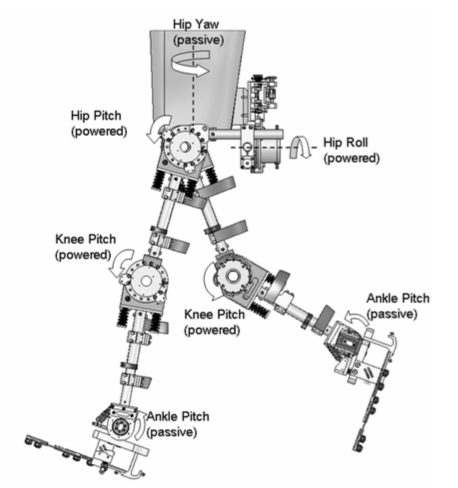
\includegraphics[width=3.in]{exos/figs/ihmc/ihmcSys}
  \caption{}
  \vspace{-0.2in}
 \label{fig:IHMCSYS}   
 \end{figure}
 
 
 \subsection{Control Specifications}
 
 Both IHMC MAE control approaches noted are relatively straight forward implementations of low-level torque control.  The first control scheme takes full advantage of the SEA actuators' ability to directly measure output torque and subsequently to perform closed-loop torque control, (see \ref{fig:IHMCTOR}). 
  \begin{figure}[thpb]
\centering
\includegraphics[width=3.in]{exos/figs/ihmc/torqueCon}
  \caption{}
  \vspace{-0.2in}
 \label{fig:IHMCTOR}   
 \end{figure}
 The controller takes in a desired torque, compares the desired value to the output torque measured at each individual actuator, then uses this value as well as its derivative to compute an actuator command signal, which in this case is a current.  The largest question in this controller, as presented in literature, is how to define the desired torque term $\tau_\text{des}$.
 
 The second low-level control approach presented in the IHMC MAE literature is a combination of a position-based controller with an inner-loop torque controller.  This control scheme is presented in Figure \ref{fig:IHMCPOS}.
  \begin{figure}[thpb]
\centering
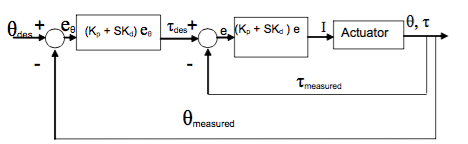
\includegraphics[width=3.in]{exos/figs/ihmc/positionCon}
  \caption{}
  \vspace{-0.2in}
 \label{fig:IHMCPOS}   
 \end{figure}
 The controller in Figure \ref{fig:IHMCPOS} shows an outer-loop position-based PD controller that takes in desired joint trajectories and compares them to measured joint positions.  These are used to generate desired torque values which are fed into an inner closed-loop torque control loop.  This control scheme is a good low-level choice if high-impedance. accurate suit motion is desired.  Similarly to the torque-only control loop above, the main question in this control scheme is how to obtain the desired joint trajectories.  
 
 One possibility for defining either the desired torques / joint trajectories in these control schemes is to use clinical gait analysis data.  With this approach, the highlighted controllers would effectively play back nominal joint trajectory data.  The foot sensors in the system would detect phase transitions, allowing the controllers to dynamically adjust the prerecorded data to the user in realtime.
 
 
 \subsection{Opinion}
 
 The design and use of series-elastic actuators is, in general, a good idea for many applications, but may be a problem for the highly dynamic maneuvers required by operators in the TALOS project.  In a large sense, bandwidth is everything in these suits due to the fact that behavior prediction is very complicated.  Simply put, 10Hz control bandwidth at the actuator may be too slow to safely react in dynamically changing environments. 
 
 The other issue with the IHMC is that it only addresses low-level control.  The designers have not specified how to generalize the process of generating torque / joint reference trajectories.  That said, other researchers do explicitly provide methods for generating desired trajectories in what amounts to a mid-level of a hierarchical control scheme.  Thus combining other approaches with the low-level, highly accuracy torque control provided by the novel SEAs presented in this section could offer a potentially good solution at the actuator level. 
 

% \end{document}


% Hian Kai Kwa and Jerryll H. Noorden and Mathew Missel and Travis Craig and Jerry E. Pratt and Peter D. Neuhaus, "Development of the IHMC Mobility Assist Exoskeleton,"  International Conference on Robotics and Automation, 2009.



%%% Local Variables:
%%% mode: latex
%%% TeX-master: "../survey"
%%% End:


% % Created 2015-09-15 Tue 11:46
% \documentclass[11pt]{article}
% \usepackage[utf8]{inputenc}
% \usepackage[T1]{fontenc}
% \usepackage{fixltx2e}
% \usepackage{graphicx}
% \usepackage{longtable}
% \usepackage{float}
% \usepackage{wrapfig}
% \usepackage{rotating}
% \usepackage[normalem]{ulem}
% \usepackage{amsmath}
% \usepackage{textcomp}
% \usepackage{marvosym}
% \usepackage{wasysym}
% \usepackage{amssymb}
% \usepackage{hyperref}
% \usepackage{color}
% \usepackage{soul}
% \tolerance=1000
% \usepackage[margin=1in]{geometry}

% \newcommand{\hilight}[1]{\colorbox{yellow}{#1}}

% %\author{Alex Ansari}
% %\date{}
% %\title{TALOS}
% %\hypersetup{
% %  pdfkeywords={},
% %  pdfsubject={},
% %  pdfcreator={Emacs 24.3.1 (Org mode 8.2.10)}}


% \begin{document}
\section{MIT Exoskeleton}

The MIT Exoskeleton is based on evidence from biology and passive walking devices that suggest that legged locomotion can be very efficient.  The main physical concept behind this efficiency being that there is a gait cycle for a pair of legs that naturally exchanges energy between gravity and inertia.  The main mechanical design principles center around the use of a combination of passive and active elements.  In particular, the MIT design uses {\bf springs, variable impedance joints, and powered actuators.}  The suit generally  functions as a lightweight, underactuated robot that runs in parallel to an operator and supports the weight of a payload. Additionally, the leg structure of the suit allows weight from the suit and payload to be transferred directly to the ground.

Of the several other design principles discussed, the MIT team emphasizes that joint {\bf powers scale linearly with mass}.  Also, the team points out that alterations in the operator's gait pattern have been shown to increase the physiological energy expended during locomotion.  Thus, the specifications for actuation and control for their system are extracted from the angle, torque , and power data of human walking joint patterns.      

\subsection{Actuator specifications}

The MIT exoskeleton uses a single actuator located at the hip.  The actuator is designed around a total system weight of 165 kg.  The maximum scaled hip torque for a system with this mass is approximately $-130$ Nm during the stance phase and approximately 100 Nm during the swing phase of the gait.  The hip is chosen as the actuated joint because proximal mass is metabolically less expensive in walking than distal mass.

The specific choice of actuation for the MIT exoskeleton hip joint was a {\bf linear series elastic actuator}.  This choice provided a lightweight and relatively inexpensive means of implementing force control with a bandwidth similar to that of natural muscle.  A model of the actuator is shown in Figure \ref{fig:mitSEA}.
\begin{figure}[thpb]
\centering
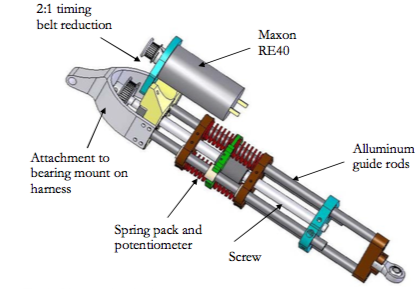
\includegraphics[width=3.in]{exos/figs/MIT/mitSEA}
  \caption{}
  \vspace{-0.2in}
 \label{fig:mitSEA}   
 \end{figure} 
Like all series elastic designs, the actuator shown in Figure \ref{fig:mitSEA} includes a spring in series with the output of the motor drive system of the actuator.  The motor-drive mechanism consists of a {\bf brushed DC motor driving a 3mm ball screw via a 2:1 reduction belt drive}.  The nut of the ball screw is coupled to the actuator output shaft via four compression die springs.  The compression of the die springs are measured using a linear potentiometer, which is how forces at the output are measured.
The team selected a {\bf 150W Maxon RE40 Brushed DC motor} for the actuator  based on the bio-mechanical data and its power and weight ratio. The force bandwidth for this actuator was characterized during both stance and swing phases of the walking gait cycle.  {\bf During stance, the bandwidth of the actuator was 35 Hz, while the bandwidth during swing was found to be 40Hz.} 
 
 \subsection{Exoskeleton Specifications}
 
 The MIT exoskeleton design has a total of fourteen degrees of freedom, three at each hip, one at each knee, two at each ankle, and one in each foot.  A cam mechanism implemented at the hip joint enables hip ab/adduction.  This system was necessary because, during abduction, there is a length difference between the operator and exoskeleton leg which results from having non-collocated centers of rotation.  The cam mechanism automatically adjusts the exoskeleton leg length such that the center of rotation of the exoskeleton hip is projected onto the biological hip center of rotation.  A picture of the MIT exoskeleton is shown in Figure \ref{fig:MITsuit}.
 \begin{figure}[thpb]
\centering
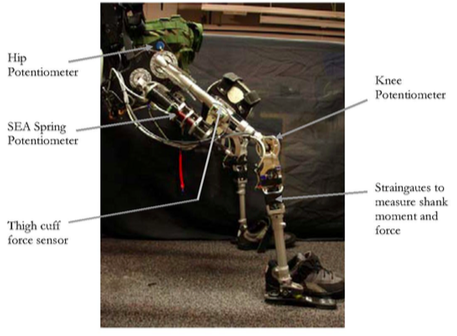
\includegraphics[width=3.in]{exos/figs/MIT/MITsuit}
  \caption{}
%  \vspace{-0.2in}
 \label{fig:MITsuit}   
 \end{figure} 
% 
 The interface between the suit and operator consists of shoulder straps, a compliant waist belt, thigh cuffs, and a shoe connection.  

 The exoskeleton implements a {\bf variable damper knee mechanism} in the flexion/extension degree of freedom using a magnetorheological damper.  The damper can exert a {\bf maximum braking torque of 60 Nm and consums on average 1W of electrical power}.  Additionally, a linear spring at the ankles captures negative energy during dorsilflexion.  The energy stored is released during plantar flexion to add energy to the system as the foot comes off the ground. A urethane spring (247 kN/m) is used as a liner spring in a lever compression assembly.  With a lever arm of 0.0381 m, the assembly yields a spring rotary stiffness of 356 Nm/rad. 
 
 A unidirectional spring assembly is also used in the hip ab/adduction degree of freedom.  The spring allows the hip to freely abduct.  The effective rotary stiffness of the spring assembly is 96 Nm/rad in order to provide the 8 Nm required during adduction.

The suit uses a 48V battery pack and is instrumented with \textbf{rotary potentiometers} at the hip and knee.  Additionally, \textbf{strain gauges} were placed on the structure of the exoskeleton shank to measured sagittal bending moment and compression force.
 
 
 \subsection{Control Specifications}
 
The MIT exoskeleton controllers use the fact that desired actuation and active damping at the knee are functions of gait cycle.  Hence, the values of these desired functions can be determined from human walking data.  Fundamentally, the control strategy works as a state machine that uses joint angle and measured forces to implement state transitions.

\begin{figure}[thpb]
\centering
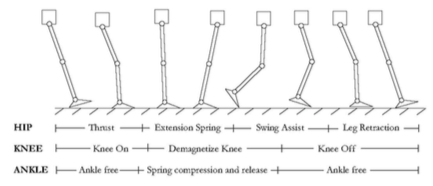
\includegraphics[width=4.in]{exos/figs/MIT/walkingCycle}
  \caption{}
  \vspace{-0.2in}
 \label{fig:walkingCycle} 
 \end{figure} 
The walking cycle around which the MIT control scheme was designed is shown in Figure \ref{fig:walkingCycle}.  The individual control strategies in the various phases of the walking cycle are highlighted in Figure \ref{fig:walkingCycle}.  For the hip there are four distinct strategies.  During the thrust phase, the hip exerts a torque that helps to raise the center of mass of the system.  During the extension spring phase, a virtual spring stiffness allows energy to be virtually stored while the center of mass moves forward.  During the swing assist phase the virtual energy is released, resulting in a torque being applied which assists in swinging the leg forward.  Finally, in leg retraction a torque is applied to help with foot placement and weight acceptance.  A diagram that illustrates how the sensors in the shank and hip joint are used to switch between these various phases is show in Figure \ref{fig:hipControl}.
 \begin{figure}[thpb]
\centering
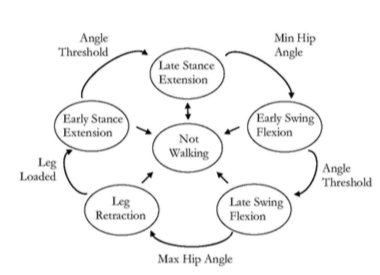
\includegraphics[width=3.in]{exos/figs/MIT/hipControl}
  \caption{}
  \vspace{-0.2in}
 \label{fig:hipControl} 
 \end{figure}  
 
 The knee controller in the MIT exoskeleton effectively functions independently from he hip controller.  During knee strike, the variable damper in the knee exerts a torque proportional to the rotational velocity of the knee joint.  A residual magnetic field remains in the knee joint after it is turned off, creating a resistive torque.  The knee therefore needs to be actively demagnetized at full extension during the last phase of stance to allow it to swing freely during the subsequent swing phase.  The state machine diagram that illustrates how the various phase transitions for the knee joint were implemented using the exoskeleton's on-board sensors is in Figure \ref{fig:kneeControl}.
  \begin{figure}[thpb]
\centering
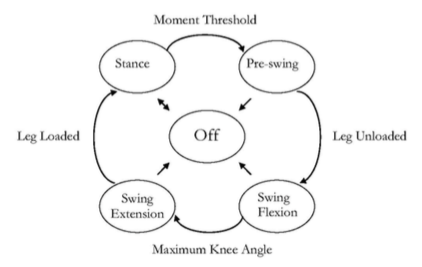
\includegraphics[width=3.in]{exos/figs/MIT/kneeControl}
  \caption{}
  \vspace{-0.2in}
 \label{fig:kneeControl} 
 \end{figure}  
  
  
%  \begin{figure}[thpb]
%\centering
%\includegraphics[width=3.in]{figs/torqueCon}
%  \caption{}
%  \vspace{-0.2in}
% \label{fig:IHMCTOR}   
% \end{figure}
% 
 
 
 \subsection{Assessment and Recommendations}
 
 The MIT hardware and control system present a very well designed and thought-out system that focuses primarily on efficiency in design.  The series elastic linear ball screw hardware design seems to be a very smart way to implement efficient drives as well as to perform high fidelity force control.  The use of a strain gauge in the shank was also a novel means of measuring ground reaction forces.  This design may offer benefits in terms of repeatability over different operators as foot fall patterns for different users may include significant variations.
 
 The details on the controllers were somewhat sparse in the sense that, at least in \cite{}, the exact means through which the added torques were derived was not provided.  Overall though, the controllers were intelligently designed in the sense that they explicitly took the biomechanics of walking into account in their design and implementation.  A similar approach for a variety of different behaviors may be very beneficial to the TALOS project.  
 
% \end{document}

% Conor James Walsh and Daniel Paluska and Kenneth Pasch and William Grand and Andrew Valiente and Hugh Herr, "Development of a lightweight, underactuated exoskeleton for load-carrying augmentation," Proceedings of the 2006 IEEE International Conference on Robotics and Automation, 2006, pp. 3485 - 3491.

% Conor James Walsh and Kenneth Pasch and Hugh Herr, "An autonomous, underactuated exoskeleton for load- carrying augmentation, " International Conference on Intelligent Robots and Systems, 2006, pp. 1410-1415.

%%% Local Variables:
%%% mode: latex
%%% TeX-master: "../survey"
%%% End:


% % Created 2015-09-15 Tue 11:46
% \documentclass[11pt]{article}
% \usepackage[utf8]{inputenc}
% \usepackage[T1]{fontenc}
% \usepackage{fixltx2e}
% \usepackage{graphicx}
% \usepackage{longtable}
% \usepackage{float}
% \usepackage{wrapfig}
% \usepackage{rotating}
% \usepackage[normalem]{ulem}
% \usepackage{amsmath}
% \usepackage{textcomp}
% \usepackage{marvosym}
% \usepackage{wasysym}
% \usepackage{amssymb}
% \usepackage{hyperref}
% \usepackage{color}
% \usepackage{soul}
% \tolerance=1000
% \usepackage[margin=1in]{geometry}

% \newcommand{\hilight}[1]{\colorbox{yellow}{#1}}

% %\author{Alex Ansari}
% %\date{}
% %\title{TALOS}
% %\hypersetup{
% %  pdfkeywords={},
% %  pdfsubject={},
% %  pdfcreator={Emacs 24.3.1 (Org mode 8.2.10)}}


% \begin{document}
\section{RoboKnee}

The RoboKnee device was built as a prototype system to enhance human strength, endurance and speed.  The main design objectoves in the RoboKnee system were to enhance human performance using a low-impedance mechanical system that incorporates a natural user interface, long life, and is comfortable to wear.  The main control objective of the suit is to provide a ``get out of the way" control scheme, wear the system inherently interacts with the user through a low-impedance interface.  

The design of a linear series elastic actuator and a novel control method for controlling a single powered joint at the knee of the operator are presented in this section.

\subsection{Actuator specifications}

The RoboKnee actuator was designed to specifically provide low impedance and high force feedback fidelity.  Series elastic actuators are a more robust option for measuring output forces and torques than using notoriously delicate and expensive load cells.  


The actuator used in the RoboKnee device is shown in Figure \ref{fig:roboAct}.  The actuator consists of a drive train subassembly and an output carriage subassembly. The two subassemblies are coupled through die compression springs.  A servo motor directly drives a ball screw assembly to drive a ball nut flange which pushes on a spring retaining plate.  Secondary spring retaining plate is coupled to an output assembly.  Measuring the deflection in the die springs makes it possible to measure the force applied to the output of the linear SEA.  
\begin{figure}[thpb]
\centering
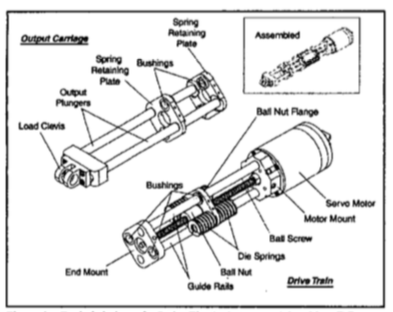
\includegraphics[width=3.in]{exos/figs/roboKnee/roboSEA}
  \caption{}
  \vspace{-0.2in}
 \label{fig:roboAct}   
 \end{figure}

The linear actuator pictured in Figure \ref{fig:roboAct} { \bf weighs 1.13 kg, has a stroke length of 30.5 cm and diameter of 5.8 cm}.  The {\bf maximum speed of the actuator is 28 cm/s}.  The actuators {\bf maximum continuous force is 565N, with a peak maximum force of 1330 N}, with {\bf maximum continuous power of 164 W, and maximum peak power of 634 W}.   

The force control bandwidth of the RoboKnee actuator is dependent on the magnitude of the force, as significant time delays can occur for larger forces due to the fact that there is an inherent time delay due to the time it takes for the spring to compress.  Thus, the {\bf small force control bandwidth of the system is 35 Hz} and the {\bf high force bandwidth is around 7.5 Hz}. 
 
 \subsection{Exoskeleton Specifications}
 
 The RoboKnee mechanism consists of a single actuated degree of freedom at the flexion/extension joint of the operator.  Note that the mechanism itslef does not provide a pathway for transferring weight from a load directly to the ground.  The mechanism transfers loads directly to the users musculoskeletal structure, and focuses primarily on augmenting the torque supplied to the users knee joint.
 
 The RoboKnee mechanism itself is composed of an off-the-shelf knee brace modified with structural pieces to extend the brace and provide actuator attachment points.  The RoboKnee mechanism is shown in \ref{fig:roboKnee}.  
 \begin{figure}[thpb]
\centering
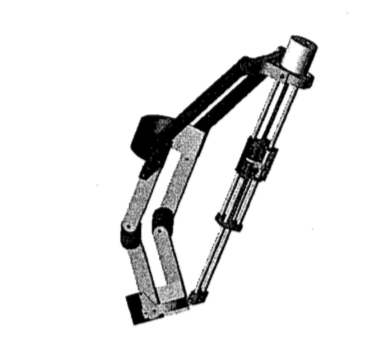
\includegraphics[width=3.in]{exos/figs/roboKnee/roboBrace}
  \caption{}
  \vspace{-0.2in}
 \label{fig:roboKnee}   
 \end{figure}
 There exact length between attachment points of the actuator is not listed in the literature, but it appears that the attachment points are at minimum the stroke displacement of the actuator  away from each other, so a {\bf minimum moment arm of 30.5 cm} is a reasonable approximation.
 
 The RoboKnee mechanism uses a linear potentiometer spanning the spring retaining plates to measure displacement in the springs and subsequently to measure force at the actuator output.  The forces between the users foot and the ground are also measured using single axis load cells.  Potentiometers which measure the knee joint angle are also employed in this design.     
 
 The single actuator as well as control and sensor electronics are run using {\bf 4 kg of nickel-metal-hydride batteries, which give the system only about 30-60 minutes of heavy use}.
 
 
 \subsection{Control Specifications}
 
 The control scheme for the RoboKnee device is a hierarchical approach, which uses a straightforward mid-level force generation scheme coupled with a low-level closed-loop force-based control loop.  The low-level, or rather joint level control is a PD control loop.
 
 The mid-level controller of the RoboKnee uses several simplifying assumptions to perform ``force amplification" to offload a percentage of the torque required by the user to actuate the system's knee joint.  This is achieved through a positive force feedback amplification which is based on measuring the ground reaction force and using this value to calculate the torque that would be required to produce this force in a static situation, namely, \[ \tau = R \times F,\] where $R$ is the vector from the ground reaction force to the users knee and $F$ is the ground reaction force.  Note that in the RoboKnee implementation this value can only be estimated due to the fact that the ankle joint angle and the ground reaction force is assumed to be purely vertical (which is a result of the single axis force sensors on the users feet).
   
   
 Once the estimated joint torque $\tau$ is calculated, an amplification factor is used in the RoboKnee control scheme to decide how much of the required knee torque will be provided by the control system.  For example, if the amplification factor were chosen to be one the actuator would completely compensate for the sensed ground reaction forces, and if it were set to zero to exoskeleton would provide no force.
  
 
 \subsection{Opinion} 
 
 The RoboKnee is a relatively simple system that highlights several intelligent hardware and control design concepts.  The use of a linear ball screw with a series elastic element that enables high-fidelity force control is a very good idea. The idea of using the measured ground reaction forces to produce the desired knee joint torque is also interesting in the sense that it is very simple and relies on a minimal amount of information.
 
 The overall design of the RoboKnee mechanism is most likely not the greatest, as it significantly increases the effective volume of the operator-system leg, but as a prototype this concept offers interesting benefits.
 
 % \end{document}
 
 % Jerry E. Pratt and Benjamin T. Krupp and Christopher J. Morse and Steven Collins, "The RoboKnee: An Exosskeleton for Enhancing Strength and Endurance During Walking," International Conference on Robotics and Automation, 2004, pp. 2430-2435.
 
 
 

\section{Conclusions and Recommendations}
\label{survey:recommend}

The (strength augmentation) exoskeletons we reviewed can be categorized into two general control categories.  The exoskeleton either directly measures user intent (e.g., from EMG data or direct human-exoskeleton interaction forces), or it estimates intent from measurements at the exoskeleton joints and applies a sensitivity amplification strategy to shadow the wearer.  

Directly measuring user intent is difficult to implement using standard sensing modalities.  For instance, EMG data is notoriously noisy and presents both modeling and calibration challenges.  It would also be extremely difficult to keep these sensors in place to obtain accurate readings in dynamic environments or combat scenarios.  For similar reasons, many systems avoid the use of load cells or complicated sensor networks to accurately obtain operator-robot interaction forces / torques.  

Sensitivity amplification strategies circumvent many of the direct operator-robot sensing issues by estimating human intent from measurements of the exoskeleton hardware. The issue with this policy is that it cannot generally distinguish between user generated torques and those produced by external sources.  As such, they end up amplifying not only the user's intent, but also external disturbances, requiring the operator to expend valuable energy to stabilize the system.  Additionally, even under the assumption that external forces can be minimized or mitigated by the user, enabling the suit to be highly responsive to perceived user intent implies that the hardware needs to be operating near the margin of stability.  This is not an optimal strategy for highly dynamic behaviors, as the suit may be pushed beyond the point to which the operator can reasonably stabilize it.

In light of these opinions, our main recommendation is that a control policy which implements a \emph{modified get out of the way} strategy would provide a reasonable strategy for dynamic exoskeleton control.  The get out of the way controller used in the Hydraulic Lower Extremity Exoskeleton discussed above would provide a starting point for this strategy.  This controller utilizes IMUs, foot contact sensors, and joint torque sensors to implement a user-reactive gravity compensating strategy.  Augmenting the sensor suit and control system to include sensors that directly measure the forces between the operator and the robot would enable this system not only avoid the user, but also to reject external disturbances.

To achieve this type of augmented get out of the way control, it may be possible to use low information density EMG (thresholded on/off muscle activation signals) with robot force/torque and angular measurements to filter operator-robot interaction forces.  As a longer term solution, we highlight research in the area of MEMs, nano-fabrication, soft sensors, etc., which has lead to the development of new, flexible ``robotic skin'' sensing arrays.  Integrating these sensing arrays into operator clothing (or attaching directly to the exoskeleton), it may be possible to directly measure human interaction forces (i.e., estimating pressure / force and exoskeleton contact locations), which was not feasible in the recent past.  Dense sensing arrays add redundancy and can improve measurement reliability.  

We also highly stress the importance of high-bandwidth control loops.  It is important that an exoskeleton's control bandwidth stays well above (typically $2-3\times$) the human control bandwidth ($2-5\,$Hz), to track dynamic motion.  Several of exoskeletons controllers are close to lower limit of this human bandwidth threshold under no-load conditions, and so can interfere in dynamic tasks.  Note that these bandwidth issues are primarily a function of the exoskeleton hardware, and thus special care/analysis needs to be given/conducted to make sure that the hardware is capable of physically producing required behaviors. 

Lastly, the importance of producing hardware that is physically capable of achieving dynamic performance is fundamentally linked to how mass is distributed throughout the system.  In general, this means that minimizing mass, more specifically distal masses on extremities, is desirable, which in turn means that at certain degrees of freedom must remain unactuated.  Underactuted control is a complicated problem which can either be ignored, in the sense that the control algorithm assumes the user will provide the necessary forces and torques for the unactuated degrees of freedom, dealt with using optimization-based control methods, or can be partially compensated using passive energy storage and dissipation elements.  Our recommendation is that a combination of biomechanically-inspired passive elements and optimization-based control methods will ultimately produce the best strategy for dealing with underactuation in higly-dynamic exoskeleton systems.


%Such feedforward, model-based controllers depend heavily on accurate exoskeleton / human dynamics and so modeling efforts must be emphasized.

% Finally, we note that 
%Many of the common model-based control methods in this survey employ feedback linearization and inverse dynamics strategies for dynamic exoskeleton control.  
%These methods (incorrectly) assume the exoskeleton is fully actuated and require users to provide certain torques at uncontrolled joints.  There are more advanced control schemes that extend to underactuated systems and may apply here (e.g., optimization-based controllers or virtual model control).  However, we note that there is a balance between feedback and feedforward control.  The better one is, the less reliant the system is on the other.
%
%Improved feedback and direct sensing of user intent / human interaction forces therefore also offers to reduce sensitivity to high accuracy models and the fully actuated assumptions in inverse dynamics control. 

%% OTHER POINTS:
% Model-based approaches are heavily reliant on accurate models 
% Underactuated -- feedback linearization typically assumes fully actuated systems.
% human bandwidth vs control bandwidth

\newpage

%%%%%%%%%%%%%%%%%%%%%%%%%%%%%%%%%%%%%%%%%%%%%%%%%%%%%%%%%%%%%%%%%%%%%%%%%%%%

\section{Appendix: Other exoskeleton systems}

\subsection{Overviews}

\url{http://powerexoskeletons.com/}\\
\url{http://exoskeletonreport.com/}\\
\url{http://robohub.org/tag/exoskeleton/}\\
\url{http://robohub.org/exoskeletons-new-and-older/}\\
\url{http://neurogadget.com/tag/exoskeleton}\\
\url{http://www.engadget.com/tag/exoskeleton/}\\
\url{http://spectrum.ieee.org/robotics/medical-robots/exoskeletons-around-the-world}\\
\url{http://spectrum.ieee.org/biomedical/bionics/the-rise-of-the-body-bots}\\
\url{http://www.extremetech.com/electronics/139633-will-we-ever-have-iron-man-exoskeletons}\\
\url{prezi.com/jygcvfxiesnm/a-brief-introduction-to-biomechanical-exoskeletons/}\\
\url{http://news.discovery.com/tech/robotics/exoskeleton-robots-top-5.htm}\\
\url{http://blog.equipoisinc.com/new-technologies-emerging-aerospace-defense-manufacturing/}\\
\url{http://nextbigfuture.com/2015/03/lower-body-exoskeleton-audi-chairless.html}\\
\url{http://www.army-technology.com/features/featuremilitary-exoskeletons-uncovered-ironman-suits-a-concrete-possibility}\\

%%%%%%%%%%%%%%%%%%%%%%%%%%%%%%%%%%%%%%%%%%%%%%%%%%%%%%%%%%%%%%%%%%%%%%%%%%%%

We do not have sufficient information to survey the following exoskeletons.\\

%%%%%%%%%%%%%%%%%%%%%%%%%%%%%%%%%%%%%%%%%%%%%%%%%%%%%%%%%%%%%%%%%%%%%%%%%%%%

\subsection{Commercial exoskeletons for augmentation}


\subsubsection{Sarcos XOS/WEAR}

\noindent
We do not have sufficient non-proprietary information to survey
this system.\\
\url{http://www.robaid.com/bionics/raytheons-second-generation-exoskeleton-xos-2.htm}\\
\url{http://techcrunch.com/2010/09/27/sarcos-xos2-the-real-life-iron-man/}\\

\subsubsection{Lockheed Martin HULC, FORTIS}

\noindent
We believe this is in collaboration with Ekso Bionics and is similar
to BLEEX.\\
\url{http://www.lockheedmartin.com/us/products/exoskeleton/hulc.html}\\
\url{http://www.lockheedmartin.com/us/products/exoskeleton/FORTIS.html}\\
\url{http://www.lockheedmartin.com/us/news/features/2014/mfc-103114-relief-daily-grind-industrial-exoskeletons-work.html}\\
\url{http://www.dailytech.com/From+HULC+to+FORTIS+the+Evolution+of+Lockheed+Martins+Incredible+Exosuit/article36421.htm}\\
\url{http://www.wired.com/2014/09/navys-exoskeleton-could-make-workers-20-times-more-productive/}\\
\url{http://robrady.com/design-project/lockheed-martin-fortis-human-powered-exoskeleton}\\
\url{http://www.cnn.com/2013/05/22/tech/innovation/exoskeleton-robot-suit/}

\subsubsection{Revision Military}

\noindent
PROWLER Human Augmentation System (HAS) Exoskeleton.\\
\url{https://www.youtube.com/watch?v=RKcqHaPhkkM}\\
\url{https://www.youtube.com/watch?v=Zq4amM9u-6o}\\

\subsubsection{Activelink/Panasonic} 

\noindent
A variety of exoskeleton products.\\
\url{http://activelink.co.jp/en}\\

Assist Suit AWN-03:\\
{\it consists of a 13-pound backpack outfitted with leg supports which allows its wearer to lift up to 33 pounds without any noticeable effort.}\\
\url{http://www.engadget.com/2015/08/20/japans-top-oil-company-is-building-an-aliens-power-loader/}\\

Power Loader Suit:\\
\url{http://pinktentacle.com/2009/09/power-loader-exoskeleton-suit/}\\
\url{http://www.extremetech.com/extreme/173463-worlds-first-affordable-powered-exoskeleton-is-almost-here-prepare-for-mech-wars}\\
\url{http://www.dealstreetasia.com/stories/panasonic-to-release-commercial-exoskeleton-to-market-in-4q-2015-9269/}\\

\subsubsection{DAEWOO}

\noindent
\url{https://www.newscientist.com/article/mg22329803.900-robotic-suit-gives-shipyard-workers-super-strength#.U9_FTPldWSp}\\
\url{http://www.geek.com/science/daewoo-dock-workers-now-using-strength-enhancing-exo-skeletons-1601290/}\\

\subsubsection{Innophys: Muscle Suit}

\noindent
Appears to be a power assist suit for lifting. Sip and puff internface?
Tokyo University of Science Prof. Hiroshi Kobayash.\\
\url{https://innophys.jp/}\\
video: \url{https://www.youtube.com/watch?v=Sqr1l909WPw}\\
video: \url{https://www.youtube.com/watch?v=mNdJgh0ZcrM}\\
video: \url{https://www.youtube.com/watch?v=NtX81pf-3G4}\\
\url{http://blogs.wsj.com/japanrealtime/2014/11/12/wearable-power-assist-device-goes-on-sale-in-japan/}

\subsubsection{Noonee (Swiss)}

\noindent
Chair exoskeleton. Passive?\\
\url{http://www.extremetech.com/extreme/188417-rejoice-commuters-and-workers-the-chairless-chair-exoskeleton-lets-you-sit-down-anywhere-anytime}\\

\subsubsection{Sagawa Electronics (Swiss)}

\noindent
Increases reach. Master exoskeleton inside larger slave exoskeleton. Running
demonstrated.\\
\url{https://www.youtube.com/watch?v=tYgHdxmCcAI}\\
\url{http://www.ohgizmo.com/2013/07/11/mk3-exoskeleton-suit-promises-to-make-schoolgirls-better-taller-stronger/}\\
\url{http://www.bitrebels.com/technology/powered-jacket-exoskeleton-japan/}\\

\subsubsection{RB-3D}

\noindent
Hercule\\
\url{http://www.rb3d.com/produits/exosquelettes/}\\


%%%%%%%%%%%%%%%%%%%%%%%%%%%%%%%%%%%%%%%%%%%%%%%%%%%%%%%%%%%%%%%%%%%%%%%%%%%%

\subsection{Academic exoskeletons for augmentation}

\subsubsection{Kanagawa Institute of Technology}

\noindent
Pneumatic exoskeleton developed at the Kanagawa Institute of Technology,
in Atsugi, Japan, allows Akiko Michihisa, a fitness trainer, ...\\
\url{http://www.ubergizmo.com/2007/10/air-pressure-exoskeleton/}\\

\subsubsection{Monash University/Chen}

\noindent
\url{http://www.dailymail.co.uk/sciencetech/article-2639939/Super-fireman-The-hi-tech-exoskeleton-firefighters-superhuman-abilities.html}\\
\url{http://news.discovery.com/tech/robotics/firefighter-exoskeleton-to-the-rescue-140521.htm}\\

%%%%%%%%%%%%%%%%%%%%%%%%%%%%%%%%%%%%%%%%%%%%%%%%%%%%%%%%%%%%%%%%%%%%%%%%%%%%

\subsection{Commercial exoskeletons for assistance and rehabilitation}

\subsubsection{ReWalk}

\noindent
On the sixth generation of this device.\\
\url{http://rewalk.com/}\\

\subsubsection{Cyberdyne}

\noindent
up to HAL 5 (already covered)\\
\url{http://spectrum.ieee.org/robotics/medical-robots/exoskeletons-are-on-the-march}\\
\url{http://www.computerweekly.com/photostory/2240108388/Photos-Cyberdyne-Hal-robotic-exoskeleton-to-help-paralyzed/7/Japan-beats-the-US-to-it-Cyberdyne-Hal-robotic-exoskeleton-to-help-paralyzed}\\
\url{http://www.dailymail.co.uk/sciencetech/article-2384930/Robotic-exoskeleton-help-rehabilitate-disabled-people-passes-safety-tests--paving-way-sale-UK.html}\\

\subsubsection{Rexbionics}

\noindent
REX exoskeleton\\
\url{http://www.rexbionics.com/}\\
\url{http://www.gizmag.com/rex-robotic-exoskeleton/15736/pictures}\\
\url{http://www.stripes.com/news/exoskeleton-could-benefit-troops-with-spinal-cord-injuries-1.113657}\\
\url{http://www.funis2cool.com/cool/rex-the-robotic-exoskeleton-could-change-the-lives-of-disabled-people.html}\\

\subsubsection{Indego/Parker Hannafin}

\noindent
Commercialization of Vanderbilt exoskeleton\\
\url{http://www.indego.com/indego/en/home}\\
\url{https://www.youtube.com/watch?v=-bYYmZNxaZk}\\
\url{http://www.roboticstrends.com/article/parker_hannifin_indego_exoskeleton}\\
\url{http://www.crainscleveland.com/article/20141112/BLOGS03/141119915/parker-hannifin-accepts-the-challenge-of-commercializing-the-indego--41951672-812546791-1442419256=:6352--}\\

\subsubsection{Honda}

\noindent
2 devicesin the walking assist program: 1) Bodyweight Support Assist and
Stride Management Assist (SMA):\\
\url{http://corporate.honda.com/innovation/walk-assist/}\\
\url{http://world.honda.com/Walking-Assist/}\\
\url{http://www.slashgear.com/honda-demo-walking-assist-exoskeleton-for-elderly-disabled-2211295/}\\
\url{http://singularityhub.com/2010/09/13/hondas-exoskeletons-help-you-walk-like-asimo-video/}\\

\subsubsection{Hyundai}

\noindent
Appears to be similar to BLEEX.\\
Article and video: \url{https://forums.xilinx.com/t5/Xcell-Daily-Blog/Hyundai-s-wearable-exoskeleton-restores-personal-mobility-to-the/ba-p/647031}\\
Hyundai's exo project is lead by Dongjin Hyun who did his
PhD with Homayoon Kazerooni at UC Berkeley and a PostDoc with Sangbae
Kim at MIT.

\subsubsection{3D Systems}

\noindent
3D printed exoskeleton. Using Ekso Bionics technology.\\
\url{http://www.dezeen.com/2014/03/05/3d-printed-exoskeleton-helps-paralysed-users-walk/}\\


\subsubsection{ExoAtlet (Russian)}

\noindent
Appears to be similar to BLEEX.\\
\url{http://robohub.org/clinical-trials-begin-for-russias-first-medical-exoskeleton/}\\

%%%%%%%%%%%%%%%%%%%%%%%%%%%%%%%%%%%%%%%%%%%%%%%%%%%%%%%%%%%%%%%%%%%%%%%%%%%%

\subsection{Academic exoskeletons for assistance and rehabilitation}

\subsubsection{Vanderbilt}

\noindent
Commercialized by Indego/Parker Hannafin/\\
\url{https://en.wikipedia.org/wiki/Vanderbilt_exoskeleton}\\
\url{http://research.vuse.vanderbilt.edu/cim/research_orthosis.html}\\
\url{http://www.dailytech.com/Iron+Man+New+Robotic+Exoskeleton+Helps+Paraplegics+Walk/article29079.htm}\\

\subsubsection{Mindwalker}

\noindent
Key feature is actuation in lateral plane.
Each of the powered joints has a series elastic
actuator, which can deliver 100 Nm torque and 1 kW power.\\
\url{https://mindwalker-project.eu/}\\
\url{http://www.3me.tudelft.nl/en/about-the-faculty/departments/biomechanical-engineering/research/dbl-delft-biorobotics-lab/exoskeleton/}\\
\url{http://www.utwente.nl/ctw/bw/research/projects/MINDWALKER/}\\
\url{http://tnsre.embs.org/2015/03/27/design-control-mindwalker-exoskeleton/}\\

\subsubsection{U. Penn}

\noindent
Student project that got some press.\\
\url{http://www.popsci.com/article/technology/invention-awards-2014-powerful-portable-and-affordable-robotic-exoskeleton}\\

\subsubsection{East China University of Science and Technology}

\noindent
Fully portable hydraulic exoskeleton. Unclear if this is for
assistance or augmentation.\\
Video: \url{http://v.youku.com/v_show/id_XMTg3MTQzNjgw.html}\\
Heng Cao: ``most difficult thing was control bandwidth'', so they
are probably not using high quality valves.
\url{http://mech.ecust.edu.cn/s/131/t/147/6a/07/info27143.htm}

\subsubsection{University of Electronic Science and Technology of China}

\noindent
Prof Hong Cheng did his Posdoc in CMU from 2006-2009 in CS.
He is very famous in China for his exoskeleton work.\\
Chinese Video: \url{http://society.kankanews.com/s/2014-12-17/0016103932.shtml}\\
\url{http://uestcrobot.net/~hcheng/}\\
\url{http://www.uestcrobot.net/?q=node/291}\\

%%%%%%%%%%%%%%%%%%%%%%%%%%%%%%%%%%%%%%%%%%%%%%%%%%%%%%%%%%%%%%%%%%%%%%%%%%%%

\subsection{Government Programs}

\subsubsection{TALOS}

\noindent
We assume you all are familiar with this program.

\subsubsection{DARPA Warrior Web}

\noindent
We assume you all are familiar with this program.

\subsubsection{Japan: NEDO}

\noindent
There was a Japanese government (NEDO) oriented project, ``Robotic
Devices for Nursing Care Project'', that intended to boost the
practical nursing care robots development, including exoskeleton.\\
\url{http://robotcare.jp/?lang=en}\\
\url{http://robotcare.jp/?page_id=29&lang=en}\\
They made a center to test the safety for robots including exoskeletons.\\
\url{http://www.rtnet-biz.jp/rtsic/}\\

\subsubsection{EU: BALANCE program}

\noindent
\url{http://balance-fp7.eu/}\\
\url{http://cordis.europa.eu/project/rcn/106854_en.html}\\

%%%%%%%%%%%%%%%%%%%%%%%%%%%%%%%%%%%%%%%%%%%%%%%%%%%%%%%%%%%%%%%%%%%%%%%%%%%%





\end{document}


Notes:

See if the Hydraulic Lower Extremity Exo is sensitivity amp and if so change opinion so we don't favor the approach.

Talk a lot about drawbacks of SEAs in IHMC.  Are these included in MIT / RoboKnee?  (low control bandwidth is mentioned in RoboKnee).  
We should have a blurb about the strengths/weakness of SEAs and possible options -- stiffer springs for force measurement and spring emulation for compliant control? 

Add references for new sensing tech
%%% Local Variables:
%%% mode: latex
%%% TeX-master: t
%%% End:
